
% this file is called up by thesis.tex
% content in this file will be fed into the main document

% ----------------------- introduction file header -----------------------
%\chapter{Search for the FCNC decay \pmb{$t\rightarrow c + Z$}}
\chapter{FCNC $tZc$ with charm-tagging}
\label{chapter:charm_tag}
This chapter presents an important fraction of my work was dedicated to the event selection using the charm-tagging techniques and
the design and optimization of the multivariate analysis.
% ----------------------- paths to graphics ------------------------

% the code below specifies where the figures are stored
\graphicspath{Chapters/CH6/figures}

\section{Event selections and reconstruction}
\label{sec:selection}
The channel studied for this work is \FCNCtZc in \ttbar decays using Soft Muon Tagging.
One of the \Pqt-quarks decays following the SM into a \PW boson and a
\Pqb-quark (called in the following \textit{SM top}), while the other
\Pqt-quark (called in the following \textit{FCNC top}) decays into a \PZ
boson and a \Pqc-quark that subsequentially decays semi-leptonically.\\
This semi-leptonic decay is tagged using the Soft Muon Tagging (SMT) technique. \\
Only the trileptonic channel is considered, i.e. the \PZ boson from the
FCNC top decays leptonically and the \PW boson from the SM top
decays leptonically.\\
Therefore the final state is characterised by the presence of three leptons, an
SMT-jet, a \Pqb-tagged jet and missing transverse momentum from the
escaping neutrinos. \\
The final states where either the \PZ or the \PW bosons decay
hadronically were not considered because of the higher backgrounds.\\
The pre-selection criteria, common to all the Signal Regions used in this work, are the following:
\begin{itemize}
	\item    Exactly three leptons (electrons or muons) required. \\
				These leptons must satisfy the requirements described in
				\cref{sec:object:el,sec:object:mu}. 
				At least one lepton must have $\pt > \SI{27}{\GeV}$. 
				The other two leptons must have $\pt > \SI{15}{\GeV}$. 
				Events with a fourth lepton with $\pt > \SI{15}{\GeV}$ are vetoed. 
	\item   There should be at least one opposite-sign same-flavour lepton pair
				(OSSF) with an invariant mass in the range 
				$|\mll - \SI{91.2}{\GeV}| < \SI{15}{\GeV}$. \\
				These two leptons are considered as the ones coming from the \PZ boson.\\ 	
				If more than one lepton pair satisfy these selections, the pair
				with the invariant mass closest to the mass of the \PZ boson is
				considered. 
\end{itemize}	

\subsection {Top quarks reconstruction}
%\begin{equation}
%\chi^2=\frac{  (m^{reco}_{j_{SMT}l_{a}l_{b}} -m_{t_{FCNC}})^2 }{\sigma^2_{t_{FCNC}}}   +\frac{  (m^{reco}_{j_{bjet}l_{c}\nu} -m_{t_{SM}})^2 }{\sigma^2_{t_{SM}}}+\frac{  (m^{reco}_{l_{c}\nu} -m_{W})^2 }{\sigma^2_{W}}
%\end{equation}

\label{sec:sel:topmassrec}
In the events having at least two jets with one of them being \Pqb-tagged, two top quarks (FCNC and SM tops) candidates are reconstructed under the FCNC \ttbar decay signal hypothesis.
The kinematics of the top-quark candidates can be reconstructed from
the corresponding decay particles.\\
The reconstructed \PZ boson is assumed to come from the FCNC top decay ($t\to cZ$),
while \Pqb-tagged jet from SM top decay ($t\to bW$).\\
In order to reconstruct both top quarks, 
further we need to associate a reconstructed jet to the \Pqc-quark from FCNC top decay, and reconstruct
the \PW boson from the SM top decay. This can be done by assuming the lepton not used to reconstruct the \PZ boson to be the one coming from the \PW boson decay,
the missing transverse momentum to be the transverse momentum of the neutrino from \PW boson decay
and determining longitudinal component of the neutrino momentum ($p^{\nu}_z$)
using the minimisation of the following expression for each jet combination:

\begin{equation}
\chi^2_{\ttbar}  =  \frac{\left(m^{\mathrm{reco}}_{j_a\ell\ell}-m_{t_{\mathrm{FCNC}}}\right)^2}{\sigma_{t_{\mathrm{FCNC}}}^2}+
\frac{\left(m^{\mathrm{reco}}_{j_b\ell_W\nu}-m_{t_{\mathrm{SM}}}\right)^2}{\sigma_{t_{\mathrm{SM}}}^2}
+ \frac{\left(m^{\mathrm{reco}}_{\ell_W\nu}-m_W\right)^2}{\sigma_W^2},
\label{eq:chi2tt}
\end{equation}
where $m^{\mathrm{reco}}_{j_a\ell\ell}$, 
$m^{\mathrm{reco}}_{j_b\ell_W\nu}$, and $m^{\mathrm{reco}}_{\ell_W\nu}$ are 
the reconstructed masses of the $cZ$, $bW$, and $\ell_W\nu$ systems, respectively.
For each jet combination, where any jet can be assigned to $j_a$, while $j_b$ must correspond to a \Pqb-tagged jet, the $\chi^2_{\ttbar}$ minimisation gives the most probable value for $p^{\nu}_z$. From all combinations, the one with the minimum $\chi^2$ is chosen.
For each event that contains at least one soft muon, the SMT-jet must be assigned to $j_a$ or $j_b$, depending on the $\chi^2$.
%This procedure assigns the SMT-jet to the \Pqc-quark from FCNC top decay or to the \Pqb-quark 
%from SM top decay (depending on the number of \Pqb-tagged jet) and determines the $p^{\nu}_z$ value, completing all ingredients to reconstruct four-momenta of the 
%top-quark candidates.
In~\Cref{eq:chi2tt}, the central value for the masses and the widths of the top quarks and \PW boson are taken from reconstructed simulated FCNC \ttbar decay signal events. This is done by matching the true \Pqc- and \Pqb-quarks in the simulated events to the reconstructed ones, setting the longitudinal momentum of the neutrino to the $p_z$ of the true simulated neutrino and then performing Bukin fits
\footnote{These fits use a piecewise function with  a Gaussian function in the centre and two 		
	asymmetric tails. Five parameters determine the overall normalization, the peak position, the width of the core, the asymmetry, the size of the lower tail, and the size of the higher tail. From these parameters, only the peak position and the width enter the $\chi^2$.}~\cite{Bukin} 
to the masses of the reconstructed top quarks and \PW boson (more details are in~\Cref{appendix:mass_resolution}). \\
The values are: 
%\begin{table}[!h]
%	\centering
%	\begin{tabular}{ll}
%		$m_{t_{\mathrm{FCNC}}}=171.2$~\GeV &  $\sigma_{t_{\mathrm{FCNC}}}=11.4$~\GeV\\
%		$m_{t_{\mathrm{SM}}}=168.0$~\GeV      &  $\sigma_{t_{\mathrm{SM}}}=23.9$~\GeV\\
%		$m_W=82.6$~\GeV									&  $\sigma_W=16.6$~\GeV\\
%	\end{tabular}
%\end{table}	
\begin{itemize}
	\item $m_{t_{\mathrm{FCNC}}}=171.2$~\GeV,  $\sigma_{t_{\mathrm{FCNC}}}=11.4$~\GeV;
	\item $m_{t_{\mathrm{SM}}}=168.0$~\GeV,  $\sigma_{t_{\mathrm{SM}}}=23.9$~\GeV;
	\item $m_W=82.6$~\GeV,  $\sigma_W=16.6$~\GeV.
\end{itemize}	
%The SM top quark candidate is reconstructed under the FCNC single-top quark production hypothesis in the events having one or two jets with exactly one being $b$-tagged,
%which is assumed to come from the top-quark decay ($t\to bW$). 
%The lepton not used to reconstruct the \PZ boson is assumed to be the one coming from \PW boson decay
%and the missing transverse momentum is assumed to be the transverse momentum of the neutrino from \PW boson decay,
%while the most probable value for the longitudinal component of the neutrino momentum is determined using the minimisation of the following expression:
%\begin{equation}
%\chi^2_{\tZ}  = 
%\frac{\left(m^{\mathrm{reco}}_{b\ell_W\nu}-m_{t_{\mathrm{SM}}}\right)^2}{\sigma_{t_{\mathrm{SM}}}^2}
%+ \frac{\left(m^{\mathrm{reco}}_{\ell_W\nu}-m_W\right)^2}{\sigma_W^2},
%\label{eq:chi2tZ}
%\end{equation}
%where $m^{\mathrm{reco}}_{j_b\ell_W\nu}$ and $m^{\mathrm{reco}}_{\ell_W\nu}$ are 
%the reconstructed masses of the $bW$ and $\ell_W\nu$ systems, respectively.
%In~\cref{eq:chi2tZ}, the central value for the masses and the widths
%of the top quark and $W$ boson are
%the same as in~\cref{eq:chi2tt}, therefore, in the events with two jets,
%the four-momentum of SM top-quark candidate reconstructed under the FCNC single-top quark
%production signal hypothesis is the same as the one
%reconstructed under the FCNC \ttbar decay signal hypothesis.\\
%The mass cuts are applied on the reconstructed top-quark candidates in the signal regions as described in the following sections.

\subsection {Signal Region definition}
\label{sec:sel:sr3}
The SR3\tZc has the following additional requirements:
\begin{itemize}
	\item At least two jets satisfying the requirements described in \Cref{sec:object:jet}. 
	\item Zero, one or two \Pqb-jets satisfying the requirements in \Cref{sec:object:bjet}. 
	\item The selected soft muon must be opposite-sign with the lepton coming from \PW boson also satisfying the requirements described in \Cref{sec:object:soft_muons} .
	\item At least one SMT jet described in \Cref{sec:object:smt}. 
	\item No requirements on the masses of both the FCNC and the SM top-quark candidates are applied. 
\end{itemize}
The event yield for each \Pqb-jet multiplicities and the total event yield is shown in Table~\ref{tab:yields:sr3}. 
Even though the selection with exactly one \Pqb-jet is the purest, for the SR3\tZc, events containing zero and two \Pqb-jet are also considered to have as many signal events as possible and then work on the separation of signal from background, as described in \Cref{sec:separation}.
\begin{table}[!h]
	\centering
	\begin{tabular}{|l|c|c|c|c|}
		\hline
		\multirow{2}{*}{\textbf{Sample}}      & \multicolumn{3}{|c|}{\textbf{Number of $b$-jets}} & \multirow{2}{*}{\textbf{Total yield}}\\
		\cline{2-4}
		& \textbf{=0}     & \textbf{=1}     & \textbf{=2}    &\\                    
		\hline   
		ZZ+LF &                 15.40 $\pm$ 0.24  & 0.41 $\pm$ 0.04   & 0.00 $\pm$ 0.00   &  15.81 $\pm$ 0.25  \\
		ZZ+HF &                 4.64  $\pm$ 0.12  & 5.15 $\pm$ 0.13   & 0.83 $\pm$ 0.03   &  10.63 $\pm$ 0.18  \\
		WZ+LF &                 20.13 $\pm$ 0.36  & 0.45 $\pm$ 0.06   & 0.01 $\pm$ 0.01   &  20.59 $\pm$ 0.37  \\
		WZ+HF &                 40.24 $\pm$ 0.51  & 21.92$\pm$ 0.38   & 3.10 $\pm$ 0.12   &  65.27 $\pm$ 0.65  \\
		VV (2l) &               0.05 $\pm$ 0.08   & 0.09 $\pm$ 0.04   & 0.00 $\pm$ 0.00   &  0.15 $\pm$ 0.09   \\
		WtZ &                   1.87 $\pm$ 0.19   & 7.80 $\pm$ 0.40   & 3.59 $\pm$ 0.26   &  13.26 $\pm$ 0.51  \\
		$t\bar{t}W$ &           0.23 $\pm$ 0.04   & 1.28 $\pm$ 0.10   & 1.04 $\pm$ 0.09   &  2.55 $\pm$ 0.14   \\
		$t\bar{t}Z$ (2l) &      0.00 $\pm$ 0.00   & 0.02 $\pm$ 0.02   & 0.00 $\pm$ 0.00   &  0.02 $\pm$ 0.02   \\
		$t\bar{t}Z$ &           7.69 $\pm$ 0.20  & 37.81 $\pm$ 0.45  & 38.35 $\pm$ 0.46   &  83.85 $\pm$ 0.67  \\
		Wt &                    0 $\pm$ 0.00      & 0.27 $\pm$ 0.19   & 0.00 $\pm$ 0.00   &  0.27 $\pm$ 0.19   \\
		tZ &                    8 $\pm$ 0.15      & 14.85 $\pm$ 0.30  & 5.60 $\pm$ 0.16   &  23.63 $\pm$ 0.37  \\
		$t\bar{t}$ &            0.91 $\pm$ 0.19   & 3.97 $\pm$ 0.39   & 1.29 $\pm$ 0.22   &  6.17 $\pm$ 0.48   \\
		Z+jets &                2.85 $\pm$ 0.80   & 1.07 $\pm$ 0.65   & 0.20 $\pm$ 0.20   &  4.12 $\pm$ 1.05   \\
		4 tops &                0.01 $\pm$ 0.00   & 0.05 $\pm$ 0.01   & 0.15 $\pm$ 0.01   &  0.20 $\pm$ 0.01   \\
		3 tops &                0.00 $\pm$ 0.00   & 0.01 $\pm$ 0.00   & 0.02 $\pm$ 0.00   &  0.03 $\pm$ 0.00   \\
		VVV &                   37 $\pm$ 0.02     & 0.11 $\pm$ 0.01   & 0.01 $\pm$ 0.00   &  0.49 $\pm$ 0.03   \\
		VH &                    5 $\pm$ 0.64      & 0.80 $\pm$ 0.57   & 0.00 $\pm$ 0.00   &  1.76 $\pm$ 0.86   \\
		$t\bar{t}H$ &           0.24 $\pm$ 0.02   & 1.37 $\pm$ 0.04   & 1.51 $\pm$ 0.04   &  3.12 $\pm$ 0.05   \\
		$t\bar{t}WW$ &          0.01 $\pm$ 0.01   & 0.09 $\pm$ 0.03   & 0.13 $\pm$ 0.03   &  0.23 $\pm$ 0.05   \\
		\hline                                                                            
		Total bkg. &            98.79 $\pm$ 1.29  & 97.53 $\pm$ 1.25  & 55.82 $\pm$ 0.64  &  252.14 $\pm$ 1.91  \\
		\hline                                                                            
		FCNC $t\bar{t}$(cZ) &        3.44 $\pm$ 0.02   & 10.65 $\pm$ 0.04  & 1.40 $\pm$ 0.02   &  15.49 $\pm$ 0.05  \\
		FCNC (c)tZ &            0.31 $\pm$ 0.02   & 1.34 $\pm$ 0.03   & 0.10 $\pm$ 0.01   &  1.74 $\pm$ 0.04  \\
		\hline                                                                                     
%		$S/\sqrt{B}$ (ctZ) &   0.38 $\pm$ 0.01           & 1.21 $\pm$ 0.02      & 0.20 $\pm$ 0.00  & 1.09 $\pm$ 0.01 \\
%		\hline		                                                                        
	\end{tabular}
	\caption{Event yield for each \Pqb-jet multiplicities and total event yield for the SR3\tZc selection.}
	\label{tab:yields:sr3}
\end{table}    
\\~\Cref{fig:sr3_kin_lep,fig:sr3_kin_jet} show the distributions of kinematic variables for events selected in the SR3 region for the \tZc coupling extraction selection (SR3\tZc).
As it can be noticed, the main background sources are \ttZ and \VVHF.

\begin{figure}[!htbp]
	\centering
	\begin{tabular}{cc}
		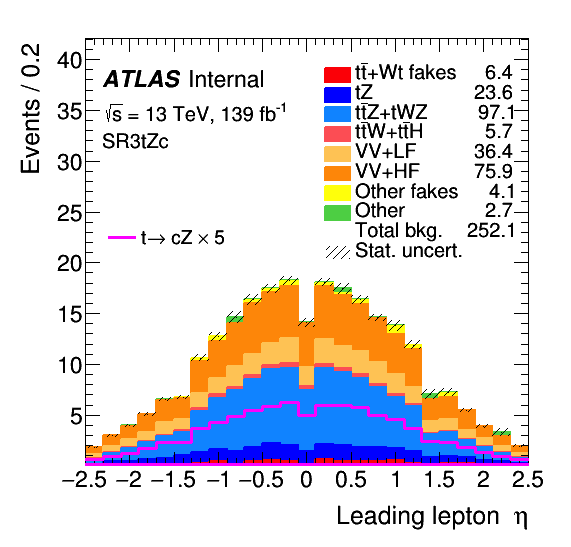
\includegraphics[width=.45\textwidth]{Chapters/CH6/figures/SR3_UsingSMT/lep1_eta} &
		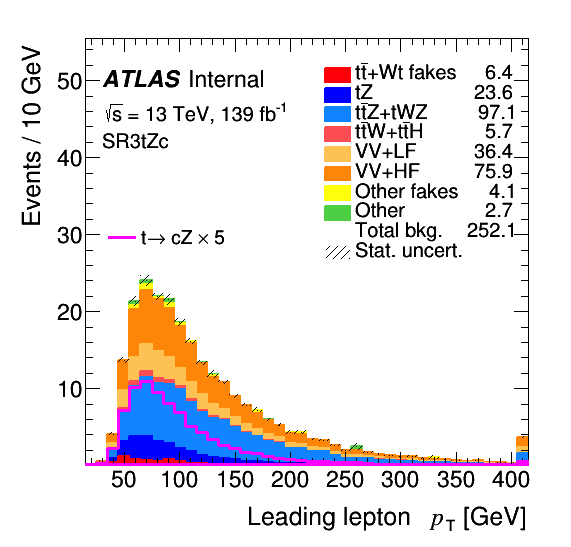
\includegraphics[width=.45\textwidth]{Chapters/CH6/figures/SR3_UsingSMT/lep1_pt} \\
		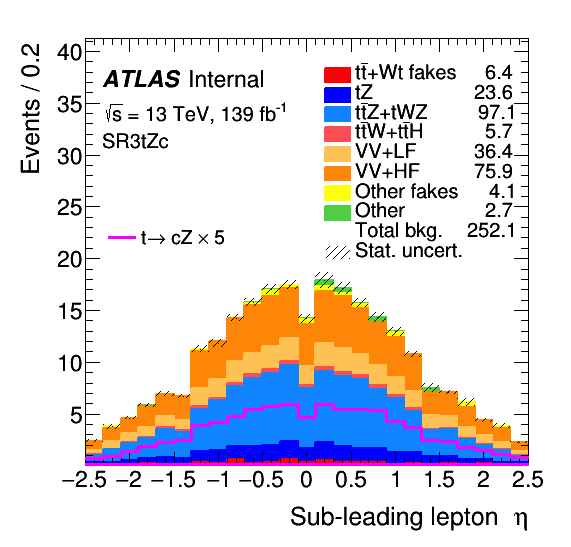
\includegraphics[width=.45\textwidth]{Chapters/CH6/figures/SR3_UsingSMT/lep2_eta} &
		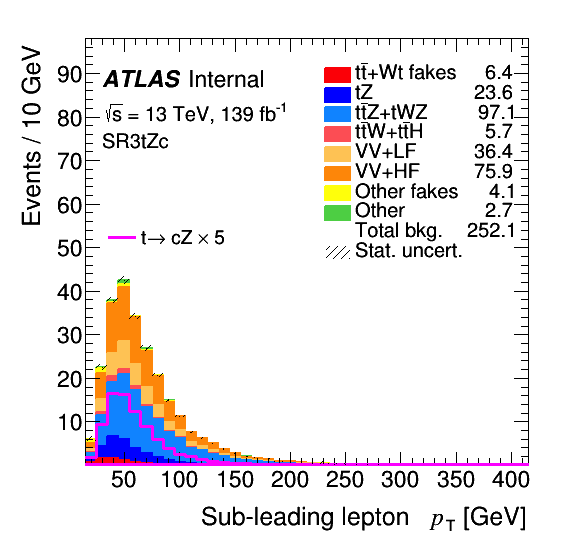
\includegraphics[width=.45\textwidth]{Chapters/CH6/figures/SR3_UsingSMT/lep2_pt} \\
		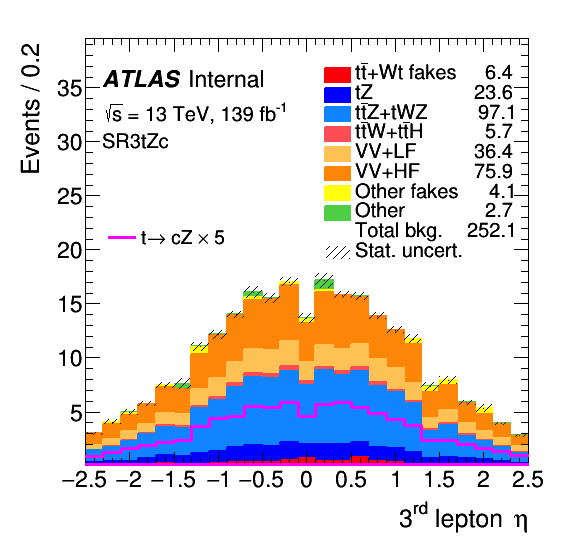
\includegraphics[width=.45\textwidth]{Chapters/CH6/figures/SR3_UsingSMT/lep3_eta} &
		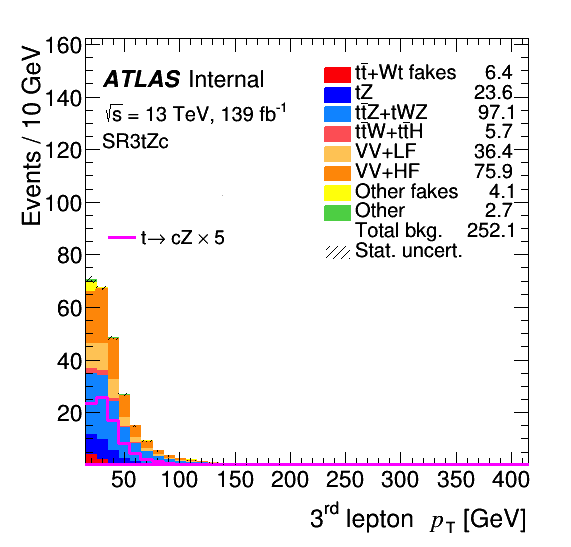
\includegraphics[width=.45\textwidth]{Chapters/CH6/figures/SR3_UsingSMT/lep3_pt} \\
	\end{tabular}
	\caption{Pre-fit distributions of kinematic variables of leptons for events selected in the SR3\tZc region.  Number of signal events are normalised to the current observed branching ratio limits and scaled by factor 5. 
		\ErrStatOnly
		\Blinded
	}%
	\label{fig:sr3_kin_lep}
\end{figure}

\begin{figure}[htbp]
	\centering
	\begin{tabular}{cc}
		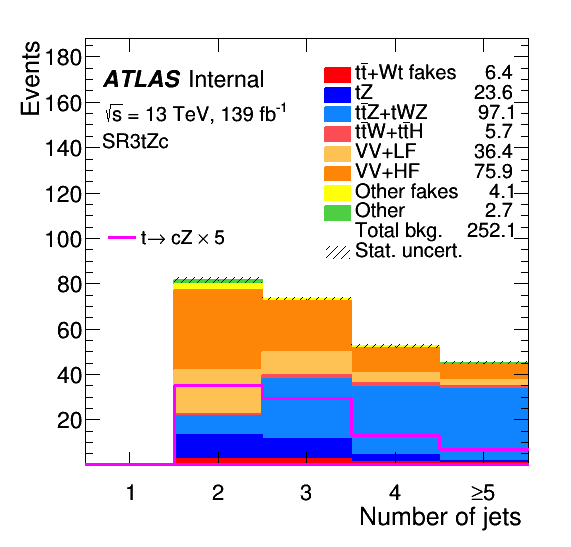
\includegraphics[width=.45\textwidth]{Chapters/CH6/figures/SR3_UsingSMT/nJets} &
	    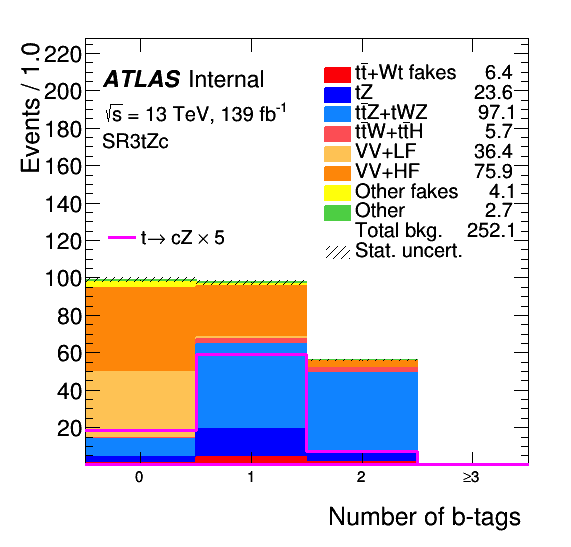
\includegraphics[width=.45\textwidth]{Chapters/CH6/figures/SR3_UsingSMT/nbJets}\\
		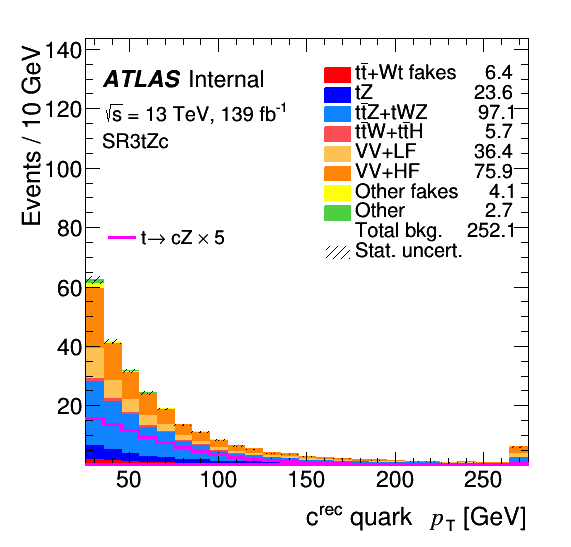
\includegraphics[width=.45\textwidth]{Chapters/CH6/figures/SR3_UsingSMT/q_pt} &
		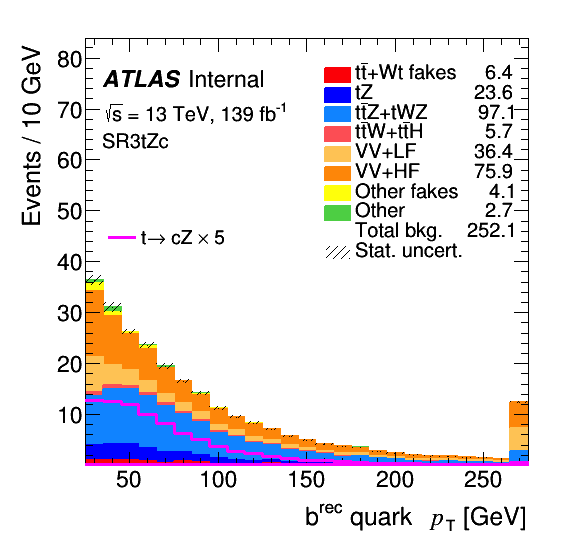
\includegraphics[width=.45\textwidth]{Chapters/CH6/figures/SR3_UsingSMT/b_pt} \\
		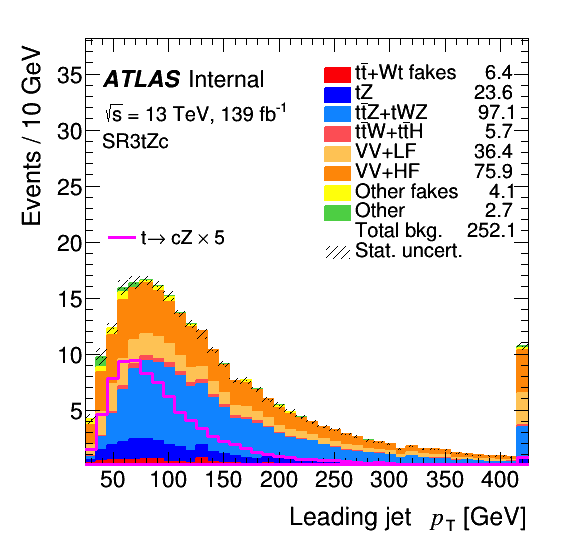
\includegraphics[width=.45\textwidth]{Chapters/CH6/figures/SR3_UsingSMT/jet_pt} &
		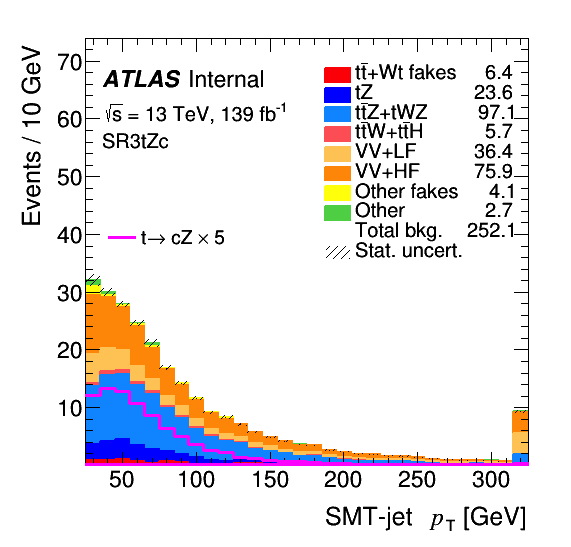
\includegraphics[width=.45\textwidth]{Chapters/CH6/figures/SR3_UsingSMT/SMTjet_Pt} \\
	\end{tabular}
	\caption{Pre-fit distributions of kinematic variables of jets for events selected in the SR3\tZc region. Number of signal events are normalised to the current observed branching ratio limits and scaled by factor 5. 
		\ErrStatOnly
		\Blinded
	}%
	\label{fig:sr3_kin_jet}
\end{figure}
\newpage
\subsection {Reconstruction of the soft muon decay chain}
\label{sec:smt_compositions}
In \ttbar events the soft muon can be originated from various sources. In MC simulation, truth information are used to identify the origin of the soft muon and the truth flavour of the SMT-jet that contains the soft muon. Therefore it is possible to reconstruct the chain of ancestors which in the end produces the soft muon. \\
Four categories of events can be identified:
\begin{itemize}
	\item muons originating from the decay chain of a b-quark produced by a $t\rightarrow Wb$ decay if the hadron and the b-quark are spatially matched within $\Delta$ R <0.4. Events with muons from b$\rightarrow \mu$, b$\rightarrow$c$\rightarrow \mu$ and b$\rightarrow \tau \rightarrow \mu$, are included in this category;
	\item muons originating from the decay chain of a c-quark produced by a $t\rightarrow cZ$ decay if the hadron and the c-quark are spatially matched within $\Delta$ R <0.4. Events with muons from c$\rightarrow \mu$ and c$\rightarrow \tau \rightarrow \mu$,   are included in this category;
	\item muons which are either produced by light hadrons coming from a top-quark decay ($t\rightarrow Wb$ or $t\rightarrow cZ$) or muons coming from the decay in flight of light hadrons, mostly pions and kaons. These muons can be also categorised as 'fake-SMT';
	\item muons that are effectively prompt leptons from a \PW or \PZ boson decay, failing the prompt lepton selection cuts, being close to a jet and therefore entering the soft muon selection criteria, referred to as prompt$\rightarrow \mu$.
\end{itemize}
According to the categories described above, Table~\ref{tab:sig_comp} shows the composition for the signal sample FCNC $t\bar{t}$(cZ). It can be noted that soft muons come from B-hadrons ($\sim$ 60\%)  and C-hadrons ($\sim$ 40\%) decays.
Table~\ref{tab:ttZ_comp} and Table~\ref{tab:VV_comp} show the composition for the main backgrounds, \ttZ and \VVHF respectively. 
For \ttZ the main contributions come from B-hadrons ($\sim$ 80\%) as expected by the \ttZ topology.
For \VVHF the main contributions come from C-hadrons ($\sim$ 60\%), mostly  \WZ\texttt{+$c\bar{c}$}.

\begin{table}[!h]
	\centering          
	\begin{tabular}{|l|c|}          
		\hline          
		\multicolumn{2}{|l|}{\textbf{FCNC $t\bar{t}$(cZ)}}    \\        
		\hline          
		\multicolumn{2}{|l|}{\textbf{Total number of events = 15.49}}    \\
		\hline
		\textbf{Chain}        									 & \textbf{Fractions $[\%]$} \\                          
		\hline          
		b$\rightarrow \mu$                 					&   15.60  \\          
		b$\rightarrow$c$\rightarrow \mu$     	&    10.16   \\          
		b$\rightarrow \tau \rightarrow \mu$  	&    0.80 \\          
		c$\rightarrow \mu$                 				 &    57.46\\          
		c$\rightarrow \tau \rightarrow \mu$  	&     0.70 \\          
		light$\rightarrow \mu$              			&    10.80  \\          
		prompt$\rightarrow \mu$                	 	&   4.48 \\            
		\hline    
	\end{tabular}    
	\caption{Reconstructed chain of ancestors that produces the soft muon for the signal sample FCNC $t\bar{t}$(cZ). The soft muon is mostly coming from B-hadrons ($\sim$ 60\%)  and C-hadrons ($\sim$ 40\%). }
	\label{tab:sig_comp}
\end{table}    
\begin{table}[!h]
	\centering          
	\begin{tabular}{|l|c|}          
		\hline          
		\multicolumn{2}{|l|}{\textbf{$t\bar t$Z}}    \\        
		\hline          
		\multicolumn{2}{|l|}{\textbf{Total number of events = 83.85}}    \\
		\hline
		\textbf{Chain}        									 & \textbf{Fractions $[\%]$} \\                          
		\hline          
		b$\rightarrow \mu$                 					&   42.24  \\          
		b$\rightarrow$c$\rightarrow \mu$     	&    31.82    \\          
		b$\rightarrow \tau \rightarrow \mu$  	&    3.01 \\          
		c$\rightarrow \mu$                 				 &    12.95\\          
		c$\rightarrow \tau \rightarrow \mu$  	&     0.14\\          
		light$\rightarrow \mu$              			&    7.32 \\          
		prompt$\rightarrow \mu$                	 	&   2.52\\            
		\hline    
	\end{tabular}    
	\caption{Reconstructed chain of ancestors that produces the soft muon for the background sample \ttZ.}
	\label{tab:ttZ_comp}
\end{table}    
\begin{table}[!h]
	\centering          
	\begin{tabular}{|l|c|}          
		\hline          
		\multicolumn{2}{|l|}{\textbf{\VVHF}}    \\        
		\hline          
		\multicolumn{2}{|l|}{\textbf{Total number of events = 75.90}}    \\
		\hline
		\textbf{Chain}        									 & \textbf{Fractions $[\%]$} \\                          
		\hline          
		b$\rightarrow \mu$                 					&   6.60  \\          
		b$\rightarrow$c$\rightarrow \mu$     	&    9.23    \\          
		b$\rightarrow \tau \rightarrow \mu$  	&    0.80 \\          
		c$\rightarrow \mu$                 				 &    57.46\\          
		c$\rightarrow \tau \rightarrow \mu$  	&     0.60\\          
		light$\rightarrow \mu$              			&    10.83 \\          
		prompt$\rightarrow \mu$                	 	&  4.48\\            
		\hline    
	\end{tabular}    
	\caption{Reconstructed chain of ancestors that produces the soft muon for the background sample \VVHF }
	\label{tab:VV_comp}
\end{table}    

\section{Background estimation}
\label{sec:background}
A variety of background sources are considered.
These include SM processes with similar final states as the FCNC \tZc
process (such as diboson or the associated production of \ttbar with
a \PZ boson), as well as events in which at least one of the leptons
in the final state is \textit{fake} (either a jet misidentified as a
lepton or a non-prompt lepton).
The estimation for the various sources of background relies on MC
simulations, for both the normalisation and the shape, while for the
\ttbar fake-lepton background the shapes are taken from MC but the
normalisation is extracted from data. \\
The \ttZ enters the event selection because of the presence in the
final state of a SM top quark and of a \PZ boson. The only difference
to the signal topology, for the semi-leptonic \ttbar decay, is the
presence of additional jets in the event. \\
The diboson background (mainly \PW\PZ and \PZ\PZ) enters the selection because of the presence
of a \PZ boson and of additional jets, that can come from heavy
quarks. 
The diboson background is split into \VVHF (heavy flavour) and \VVLF (light flavour) based on the types of jets associated:
if one of the associated jets originated from \Pqb-quark or \Pqc-quark then it is considered as \VVHF, otherwise it is considered as \VVLF. % chktex 13
The jet type is determined using the \texttt{jet\_truthflav} variable.
This variable, provided by the flavour tagging group, defines a cone of $\Delta R < 0.3$ associated with each jet.
If a \Pqb-hadron with ( \pT > \SI{5}{\GeV}) is found within this cone the jet is identified as a \bjet.
If no \Pqb-hadrons are found, the algorithm searches for \Pqc-hadrons, then \Pgt leptons.
If none of these identifiers are found the jet is labelled as a light jet.\\

%\clearpage
%\subsection {Fake composition}
%The origin of the three leptons from \ttbar events was studied, to
%understand where the fake leptons come from and eventually define an
%uncertainty to take into account the different sources in the signal
%and control regions. The origin of the three leptons from \ttbar
%events is shown in \cref{fig:bkg:fakes:ttbar:comp}. As it can be
%seen, apart from the leptons for which the mother is the top quark
%(\SI{66}{\%} of the leptons in each event), the fake leptons come from
%either photon conversions (around \SI{5}{\%}, depending on the region)
%or from \Pqb-hadrons (around \SI{25}{\%}, depending on the region). \\
%Some differences can be noticed for the photon conversion and
%\Pqb-hadron fractions in the signal regions with respect to the \ttbar
%control region where the \ttbar background is controlled. To take into
%account this differences, a systematic uncertainties is added. 
%
%\begin{figure}[htbp]
%	\centering
%	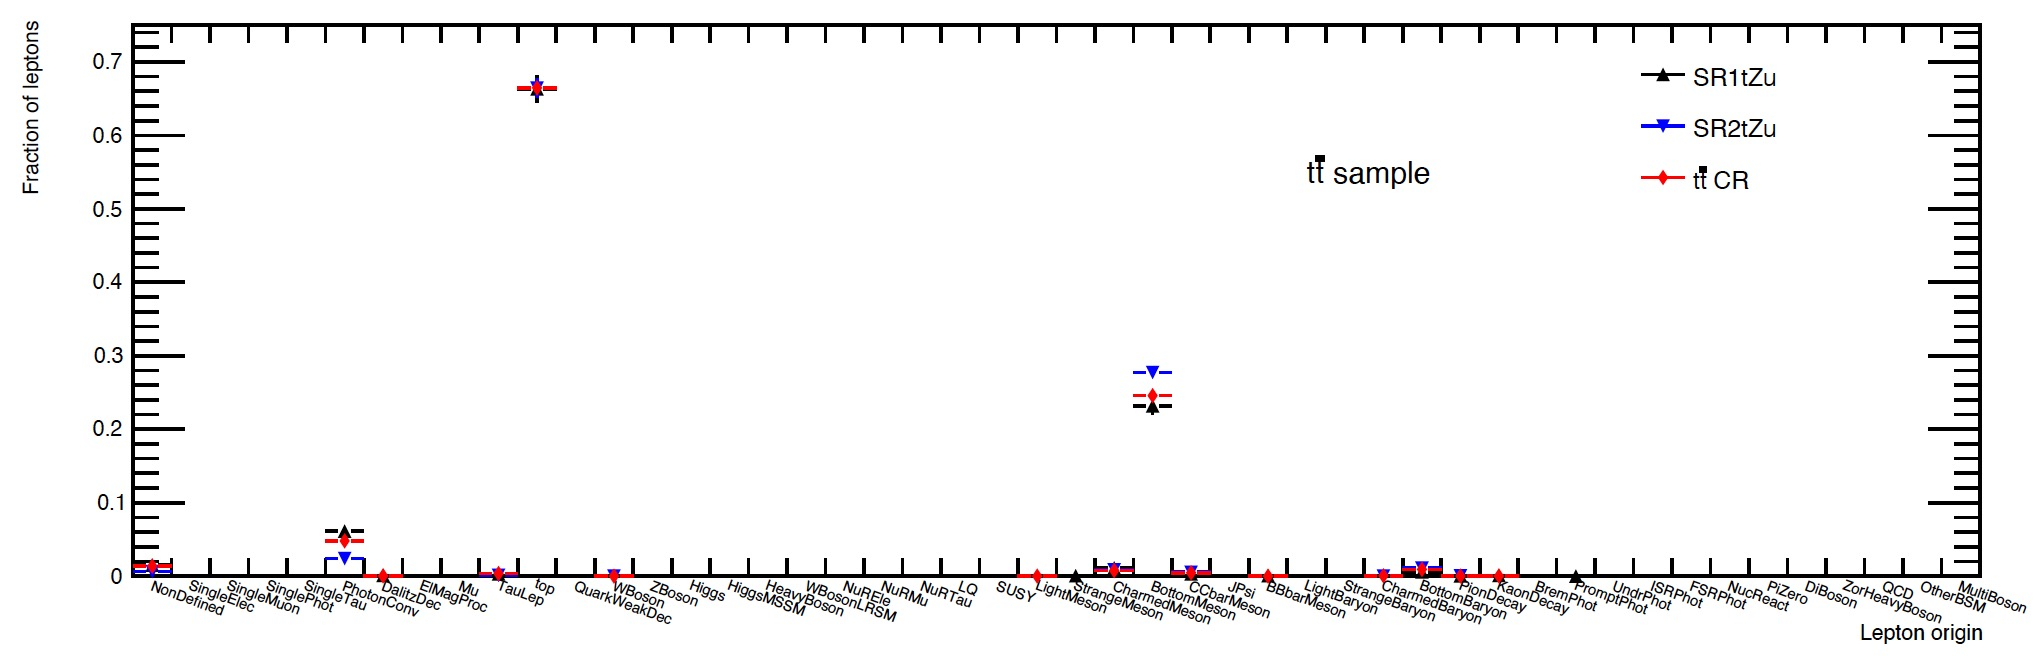
\includegraphics[width=1.\textwidth]{Chapters/CH6/figures/ttbar_leptons_origin}
%	\caption{Origin of the three leptons from \ttbar events in the
%		SR1\tZu, SR2\tZu and \ttbar CR. 
%	}%
%	\label{fig:bkg:fakes:ttbar:comp}
%\end{figure}
%
%\clearpage
%\FloatBarrier


\section{Separation of signal from background events}
\label{sec:separation}
A multivariate analysis (MVA) technique is used to separate signal from background. 
The Gradient Boosted Decision Trees (GBDT) method with TMVA software package 
is exploited in this study~\cite{BDTG,TMVA}. The GBDT output score is in the range between -1 and 1.
The most signal-like events have scores near 1 while the most background-like events have scores near -1. The GBDTs are trained separately in each signal regions as described below.
The SR3\tZc is defined targeting the FCNC \tZc coupling in \ttbar decay events
using the soft muon tagging, therefore the MVA discriminant for this coupling, \Dthree,  is built using the GBDT trained with the FCNC \tZc \ttbar decay events against backgrounds.

\subsection {Input variables}
A set of variables as the GBDT input is used to train and test the GBDT method on the events in
each signal region. Those variables are listed in \Cref{tab:D3input}, ordered by the separation value, defined by, as in~\cite{TMVA}:
\begin{equation*}
\langle s^{2}\rangle = \frac{1}{2}\int \frac{[p_{s}(y)-p_{b}(y)]^{2}}{p_{s}(y)+p_{b}(y)}dy
\end{equation*}
where $p_{s}(y)$ and $p_{b}(y)$ are the signal and background PDFs of the classifier $y$. 
The separation is 0 (1) for identical (non-overlapping) signal and background shapes.\\
These sets of input variables are constructed based on separation values, correlations and impact on the BDT performance. The details are documented in Appendix~\ref{app:BDT}.  
The distributions of input variables in each signal region are presented in~\Cref{fig:separation:SR3}.

\begin{table}[!htbp]
	\small
	\centering
	\begin{tabular}{ccc}
		\toprule
		Variable & $\langle s^{2}\rangle$  & Definition \\
		\midrule
		$m_{b\ell\nu}$  &  0.1717  &  SM top-quark candidate mass  \\
		$N\,b\,jets$  &  0.08218  &  Number of b-jets tagged with DL1r  \\
		$m_{q\ell\ell}$  &  0.07019  &  FCNC top-quark candidate mass  \\
		$\frac{\mu^{soft} ID p_{T}}{SMT\,jet\,Sum p_{T} Trk}$  &  0.03357  &  Ratio between the soft muon ID pT and pT sum of tracks  \\
		$\Delta R(\ell,Z)$  &  0.03141  &  $\Delta R$ between $W$ boson lepton and $Z$ boson candidates  \\
		$\Delta R(t_{\text{SM}},t_{\text{FCNC}})$  &  0.02508  &  $\Delta R$ between SM and FCNC top-quark candidates  \\
		$\Delta R(\mu^{soft},Z)$  &  0.006596  &  $\Delta R$ between soft muon and $Z$ boson candidates  \\
		\bottomrule
	\end{tabular}
	\caption{
	Set of variables used in the training of the GBDT in SR3\tZc to built the \Dthree discriminant used in the \tZc coupling search. Variables are ordered by the separation 	$\langle s^{2}\rangle$ value. }
	\label{tab:D3input}
\end{table}

\subsection {GBDT training and evaluation}
In order to train the GBDT algorithm and have a reliable model with a good performance, it is better to use as much statistics as possible from the available signal and background MC samples.
On the other hand, to check the performance and validate the model, 
the trained GBDT model must be applied on the test sample (events that are not used in the training phase) that has sufficiently large statistics. 
Therefore, \SI{80}{\%} of available MC statistics is used for the training while \SI{20}{\%} 
for the testing, as described below.\\
All samples, including MC systematics samples and data (currently only in CRs), are divided into five approximately equal size groups using pseudo-random numbers%\footnote{A pseudo-random number is generated for each event using the \texttt{C++ srand} generator with the sum of the dataset \texttt{RunNumber}, \texttt{DSID} and \texttt{EventNumber} as seed.}
, which 
ensures that the same event in nominal samples %and systematics samples%\footnote{For example, the sample with varied jet energy resolution.} 
is assigned in the same group.  
All events in each group have assigned the same integer pseudo-random number from 1 to 5.\\ 
Five equivalent GBDT models are trained using four groups of nominal MC samples. 
Each training uses different combination of four groups out of five. 
The remaining one group is used as a test sample.
Each of five GBDTs is evaluated on events with the assigned pseudo-random number
that is not assigned to the training events of that GBDT. \\
\Cref{tab:BDTparam} shows the values for configuration options of the BDT method.
They are chosen to counteract overtraining
and have an optimal performance.
\begin{table}[!htbp]
%	\small
	\centering 
	\begin{tabular}{cc}
		\toprule
		Option & Value for \Dthree \\
		\hline
		NTrees & 800 \\ 
		MinNodeSize & 2\% \\
		BoostType & Grad \\
		Shrinkage & 0.05 \\
		UseBaggedBoost  & True \\
		BaggedSampleFraction & 0.6\\
		nCuts  & 200 \\
		MaxDepth &  2\\
		NegWeightTreatment & IgnoreNegWeightsInTraining\\
		\bottomrule
	\end{tabular}
	\caption{
	Used values for configuration options of the TMVA method Boosted Decision Trees~\cite{TMVA}. 
}%
\label{tab:BDTparam}
\end{table}

\subsection {GBDT performance and overtraining checks }
Overtraining  leads  to  a  seeming  increase  in  the  classification performance  over  the
objectively  achievable  one,  if  measured  on  the  training  sample,  and  to  an  effective
performance decrease when measured with an independent test sample.  A convenient way to detect overtraining and to measure its impact is therefore to compare the performance results between training and test samples. \Cref{fig:separation:SR3:ROC} present the Receiver Operating  Characteristic (ROC) curves for each GBDT output score in the signal region, while \Cref{fig:separation:SR3:GBDTbkg} show the GBDT output score distributions for signal and background samples, comparing results between training and test samples.
No significant overtraining is detected. The GBDT output scores for each of five BDTGs used to
built discriminant variables are compared in~\Cref{fig:separation:GBDT}.  %The GBDTs suffer from low background MC statistics, however results seem to be fairly stable within the statistical uncertainties. 
\\Input variables importance for each GBDT are presented in~\Cref{tab:D3importance}. The importance is evaluated as the total separation gain that this variable had in the decision trees (weighted by the number of events). It is normalized to all variables together, which have an importance of 1.
\begin{table}[!htbp]
	small
	\centering
	\begin{tabular}{cccccc}
		\toprule
		Variable & GBDT \#1 & GBDT \#2 & GBDT \#3 & GBDT \#4 & GBDT \#5 \\
		\midrule
		$m_{q\ell\ell}$  &  0.1807  &  0.1758  &  0.1795  &  0.1799  &  0.1767  \\ 
		$\Delta R(\mu^{soft},Z)$  &  0.1613  &  0.1597  &  0.1603  &  0.1555  &  0.1616  \\ 
		$\Delta R(t_{\text{SM}},t_{\text{FCNC}})$  &  0.161  &  0.1635  &  0.1598  &  0.1634  &  0.1635  \\ 
		$m_{b\ell\nu}$  &  0.1536  &  0.1566  &  0.1565  &  0.1642  &  0.1478  \\ 
		$\Delta R(\ell,Z)$  &  0.1359  &  0.1433  &  0.1399  &  0.1378  &  0.1446  \\ 
		$\frac{\mu^{soft} ID p_{T}}{SMT\,jet\,Sum p_{T} Trk}$  &  0.1216  &  0.1179  &  0.122  &  0.1203  &  0.1216  \\ 
		$N\,b\,jets$  &  0.08582  &  0.08308  &  0.08205  &  0.07875  &  0.08431  \\ 
		\bottomrule
	\end{tabular}
	\caption{
	Input variables importance in each GBDT used to built the \Dthree discriminant.
}%
\label{tab:D3importance}
\end{table}

\begin{figure}[htbp]
	\centering
	\begin{tabular}{cc}
		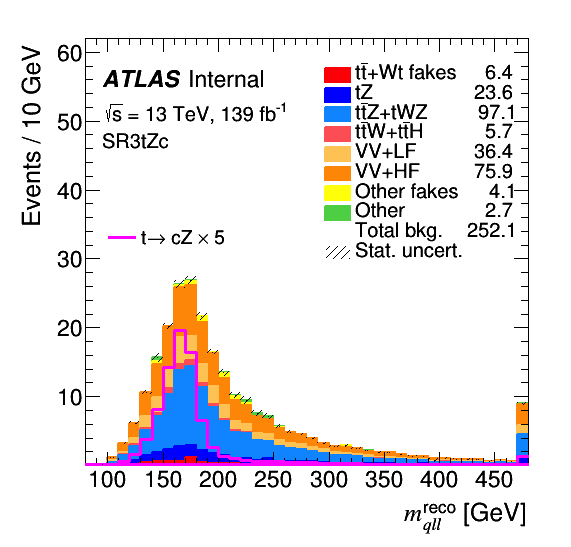
\includegraphics[width=.45\textwidth]{Chapters/CH6/figures/SR3_UsingSMT/tFCNC} &
		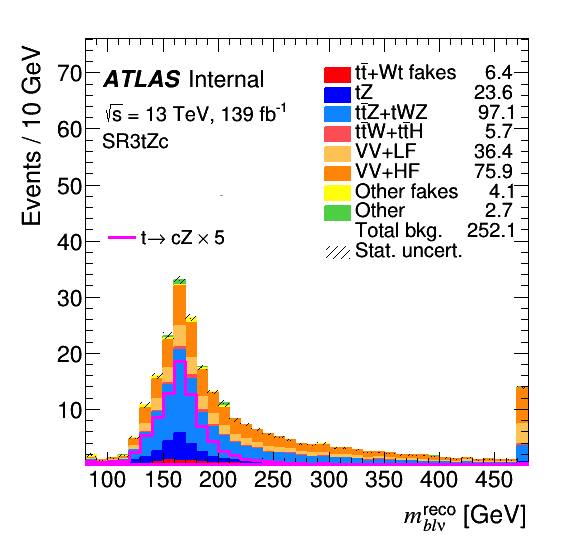
\includegraphics[width=.45\textwidth]{Chapters/CH6/figures/SR3_UsingSMT/tSM} \\
		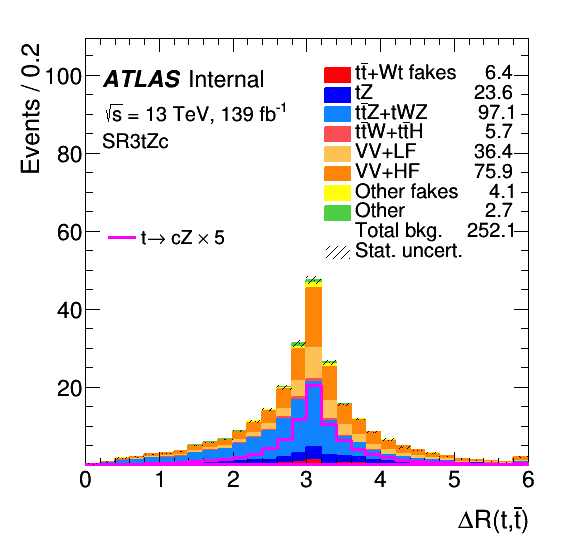
\includegraphics[width=.45\textwidth]{Chapters/CH6/figures/SR3_UsingSMT/ttbar_dR} &
		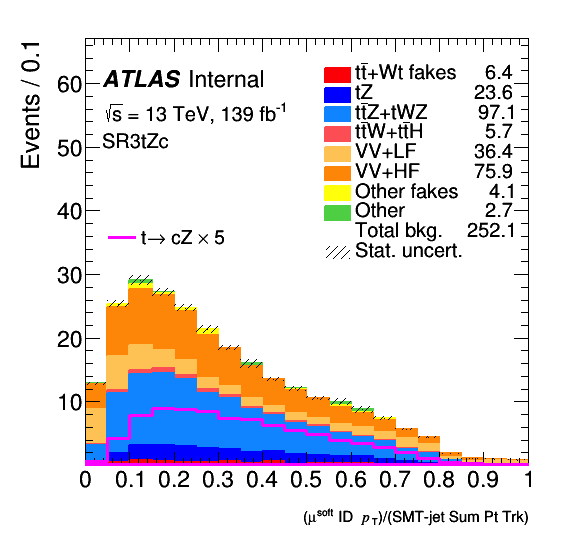
\includegraphics[width=.45\textwidth]{Chapters/CH6/figures/SR3_UsingSMT/softmu_pt_id_SumPtTrkPt500} \\
		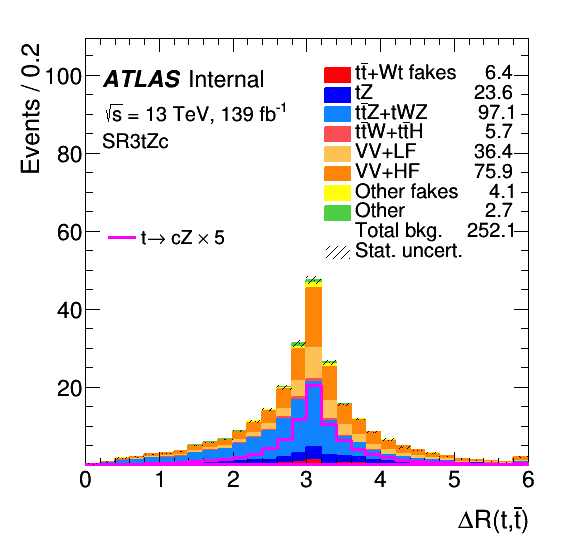
\includegraphics[width=.45\textwidth]{Chapters/CH6/figures/SR3_UsingSMT/ttbar_dR} &
		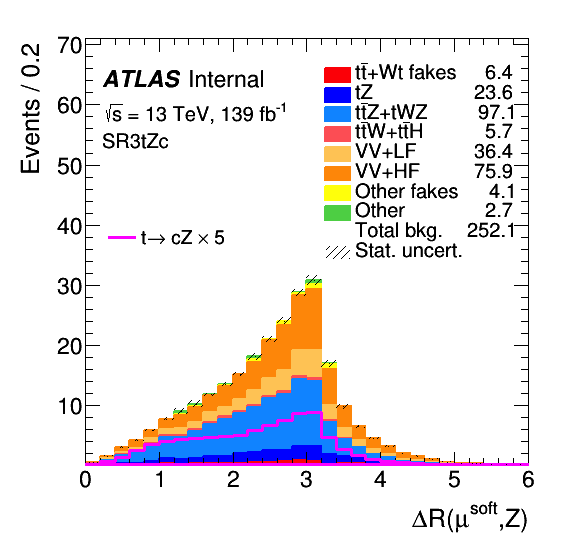
\includegraphics[width=.45\textwidth]{Chapters/CH6/figures/SR3_UsingSMT/softmuZ_dR} \\
	\end{tabular}
	\caption{Pre-fit distributions of the input variables used in the training of the GBDT in SR3\tZc to built the \Dthree discriminant. Number of signal events are normalised to the current observed branching ratio limits and scaled by factor 5.  
		\ErrStatOnly
		\Blinded
	}%
	\label{fig:separation:SR3}
\end{figure}

\begin{figure}[htbp]
	\centering
	\begin{tabular}{ccc}
		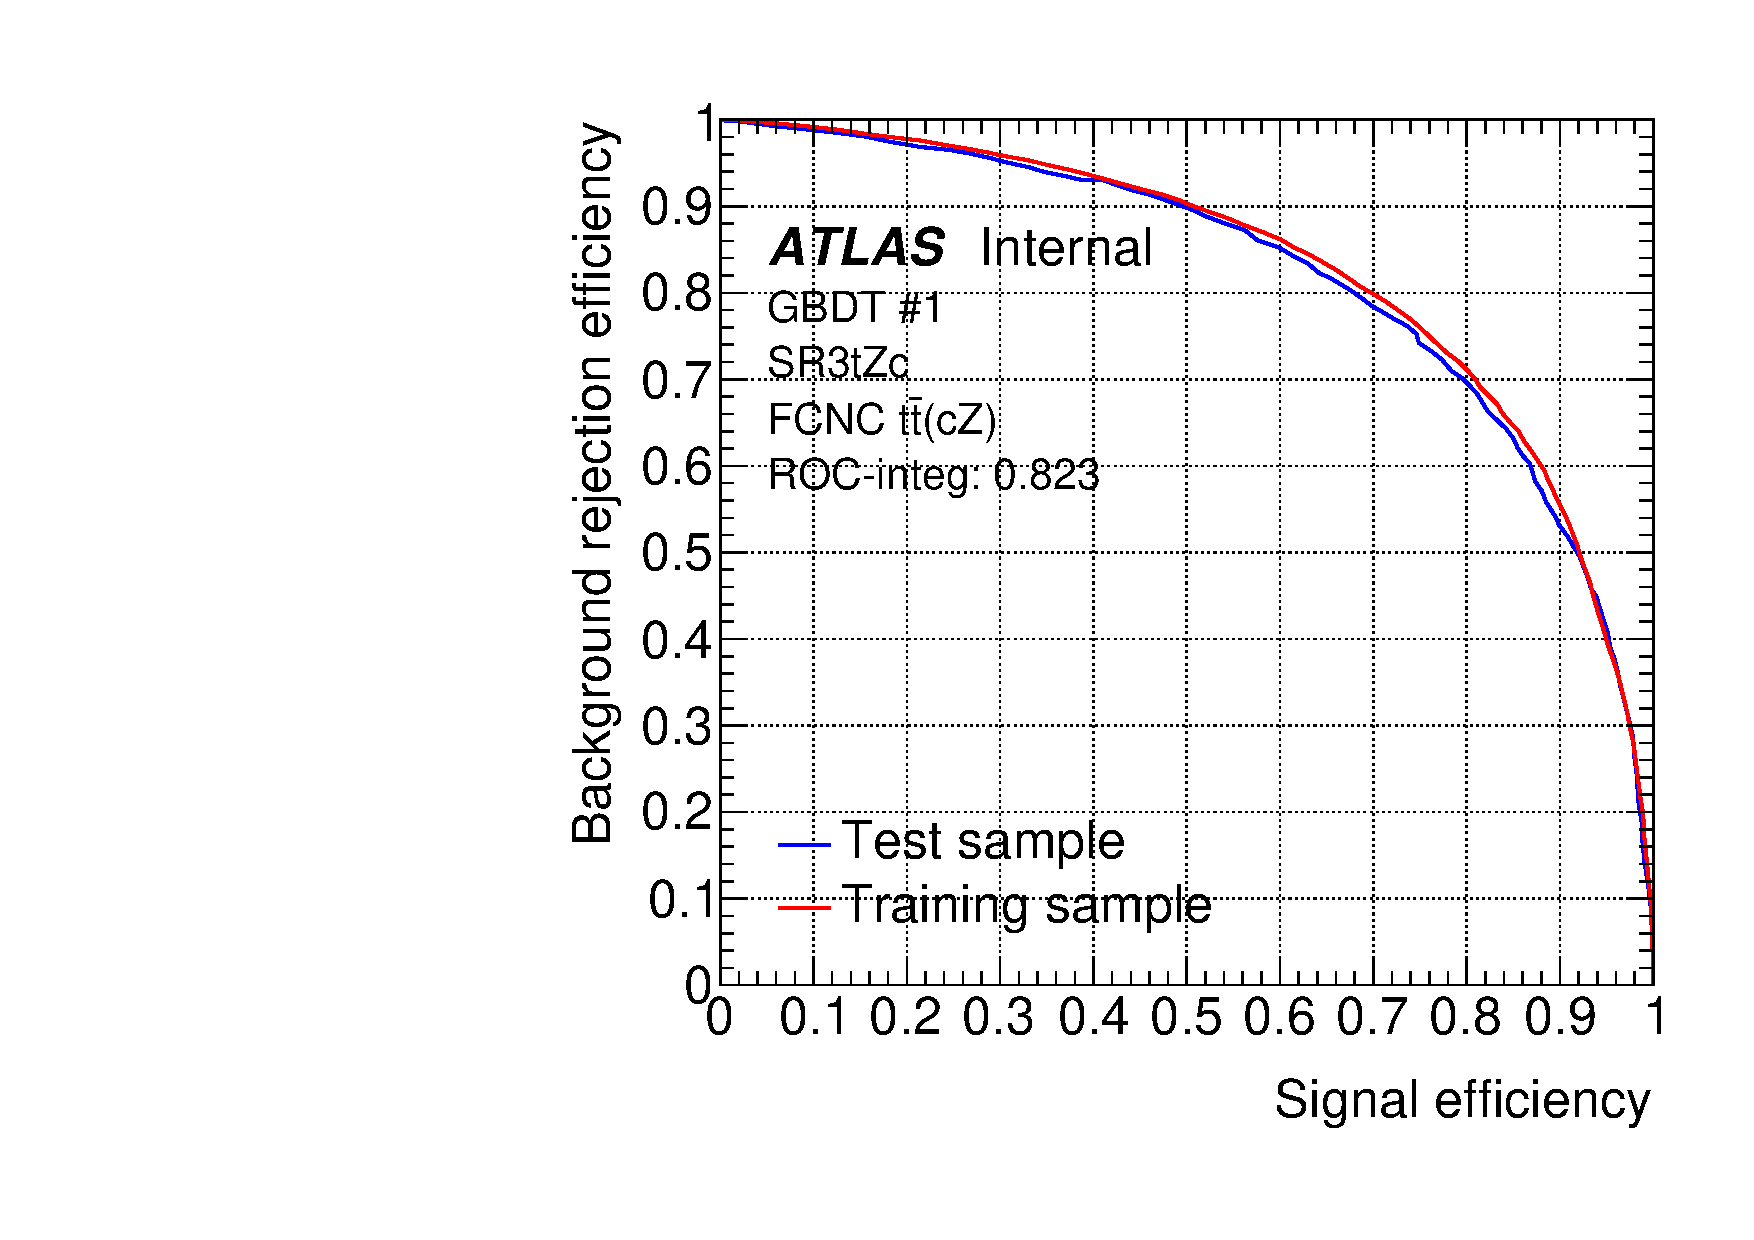
\includegraphics[width=.3\textwidth]{Chapters/CH6/figures/SR3_UsingSMT/BDT/ROC_Fold1} &
		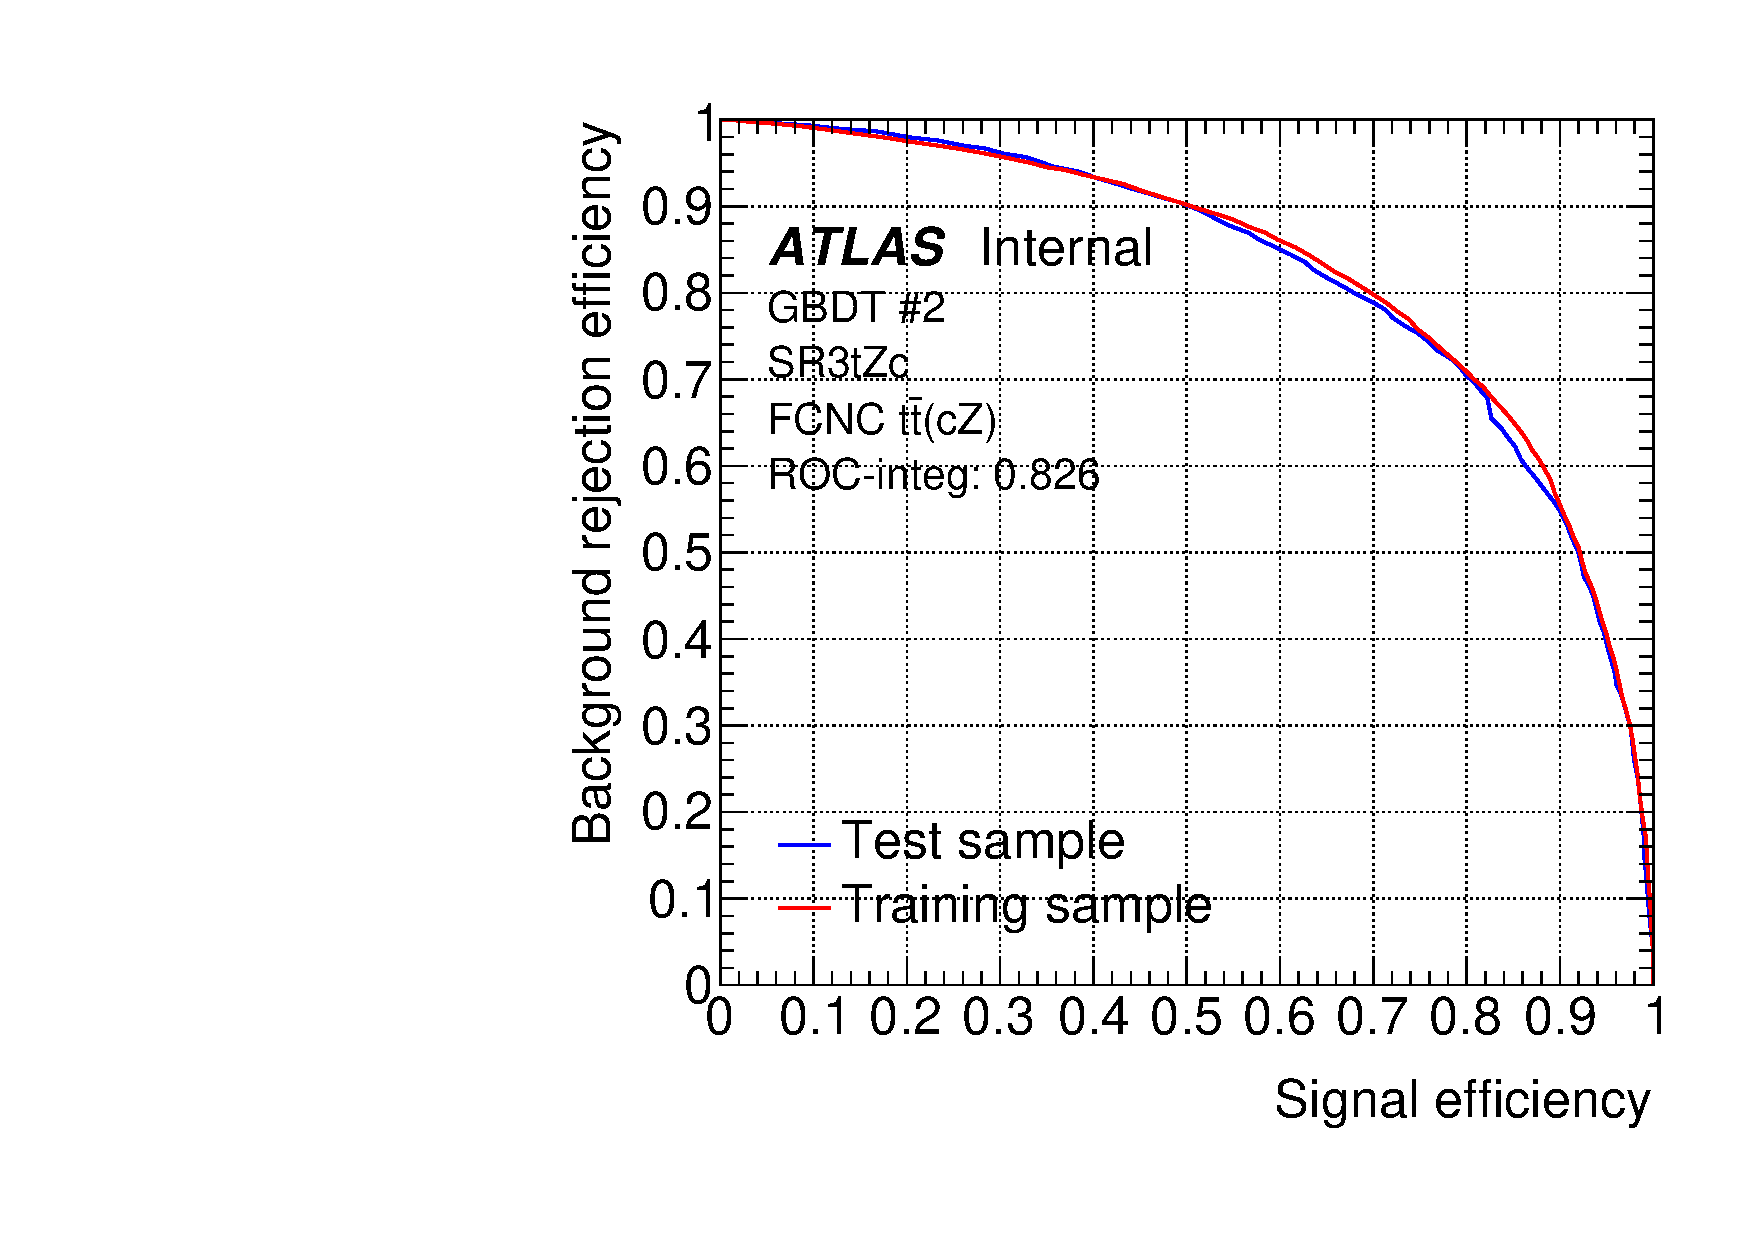
\includegraphics[width=.3\textwidth]{Chapters/CH6/figures/SR3_UsingSMT/BDT/ROC_Fold2} &
		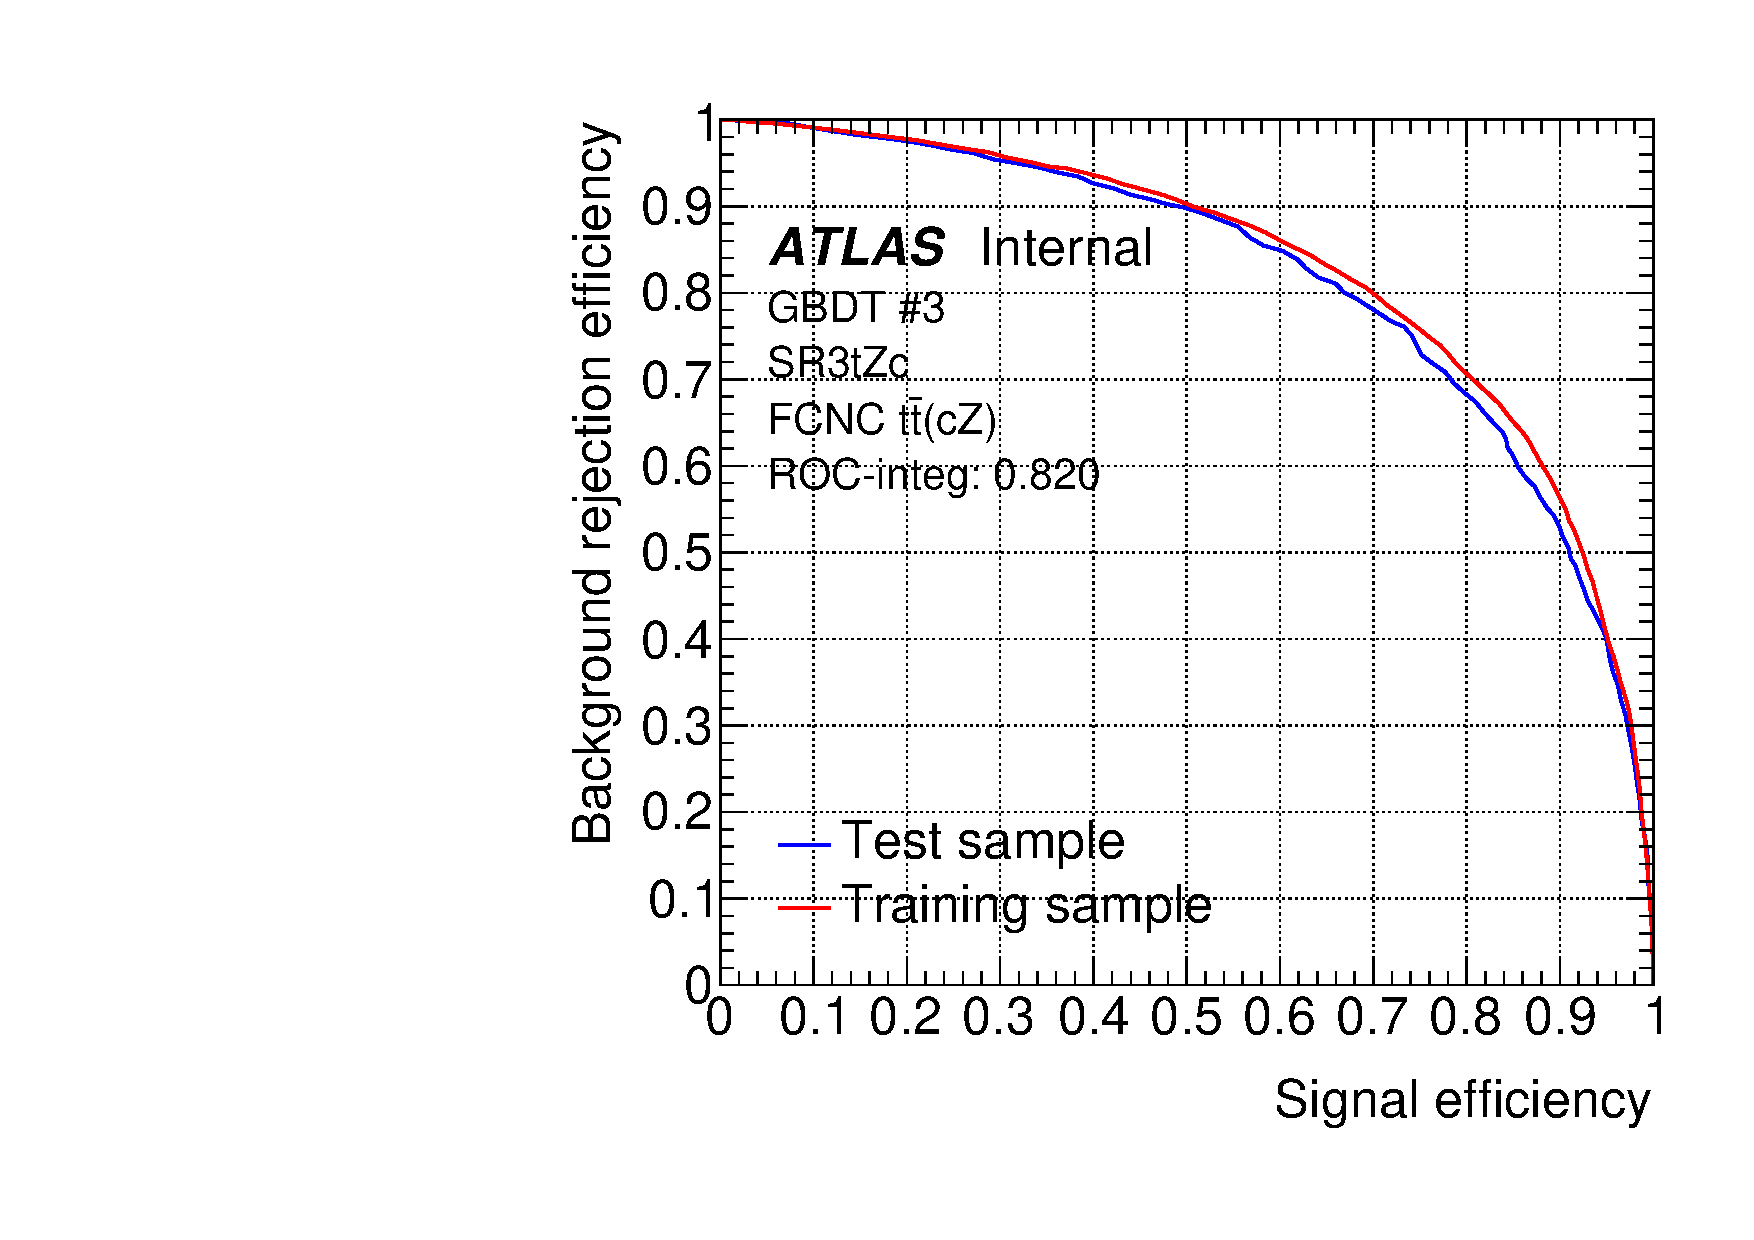
\includegraphics[width=.3\textwidth]{Chapters/CH6/figures/SR3_UsingSMT/BDT/ROC_Fold3} \\ 
		\multicolumn{3}{c}{
			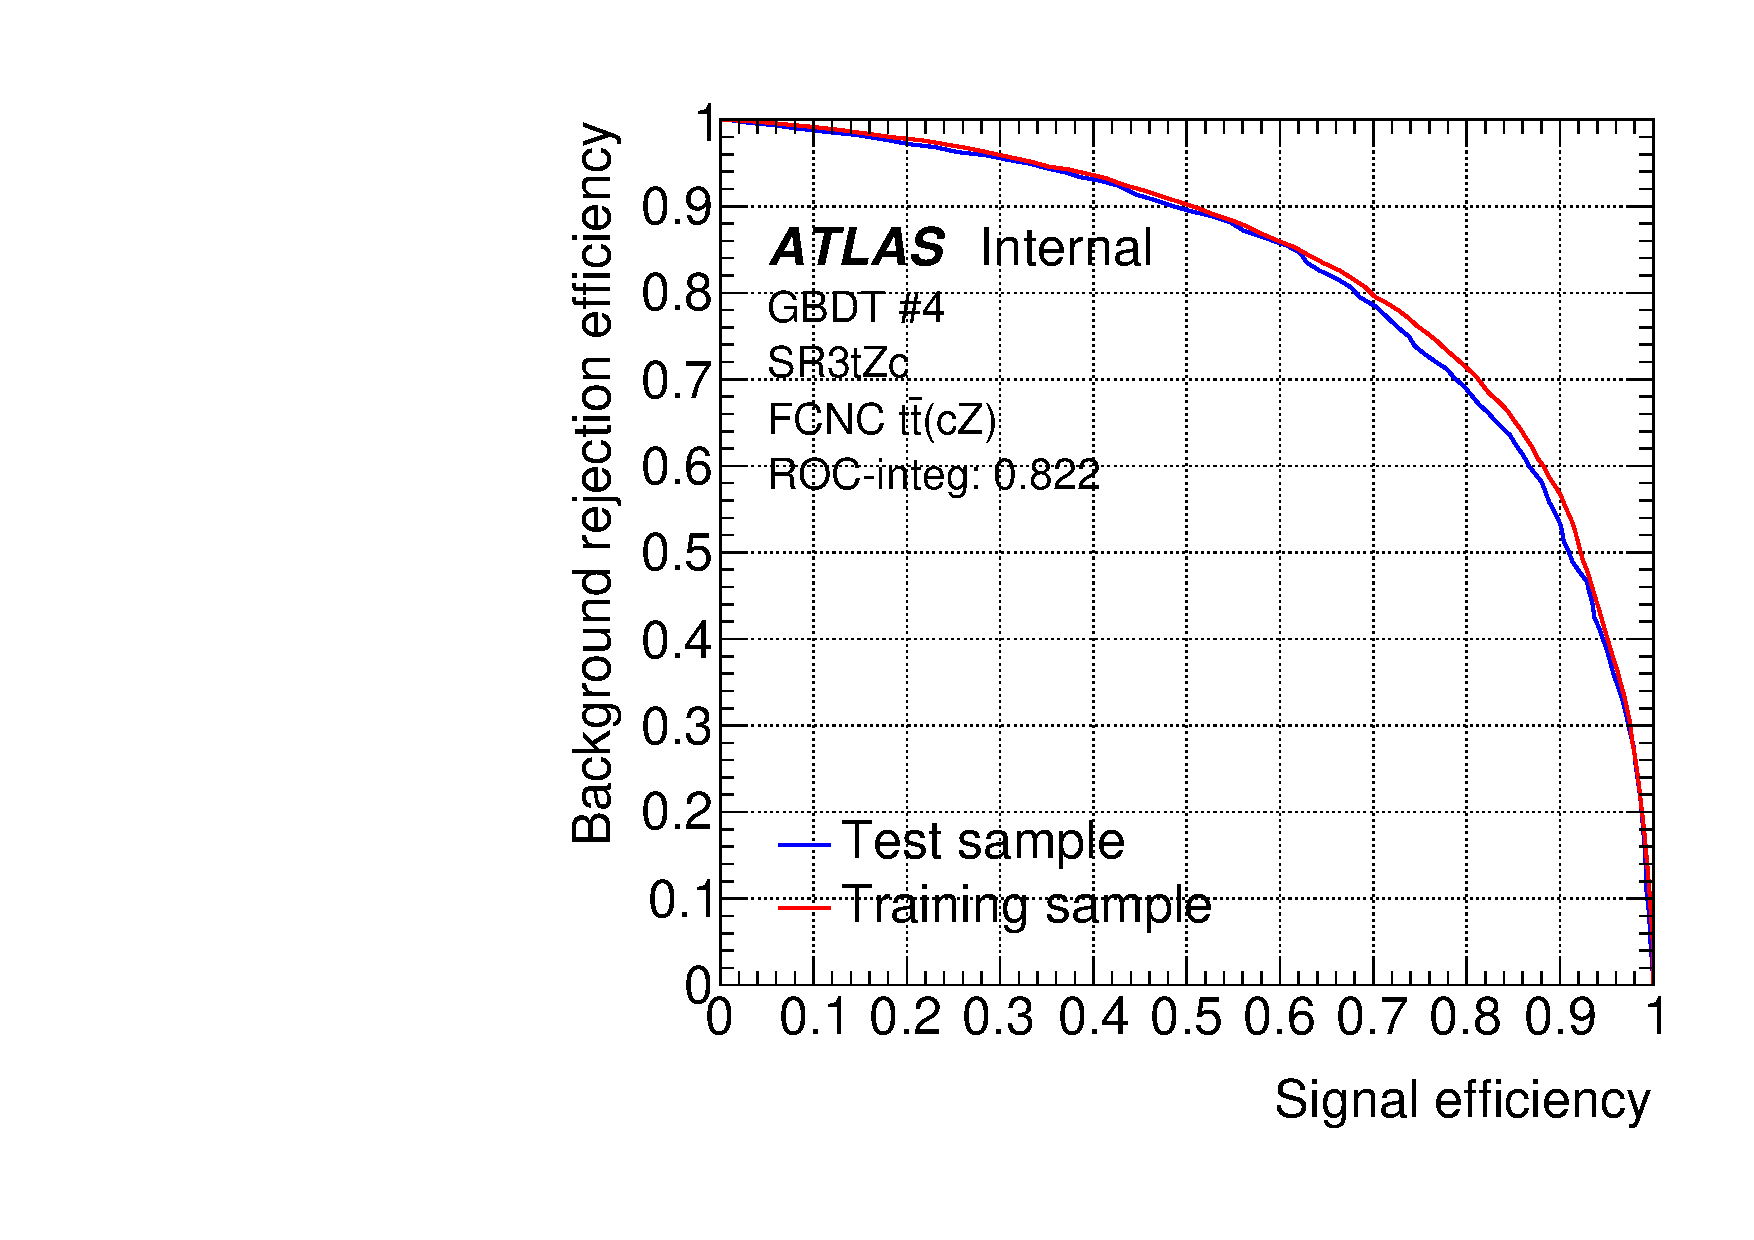
\includegraphics[width=.3\textwidth]{Chapters/CH6/figures/SR3_UsingSMT/BDT/ROC_Fold4}
			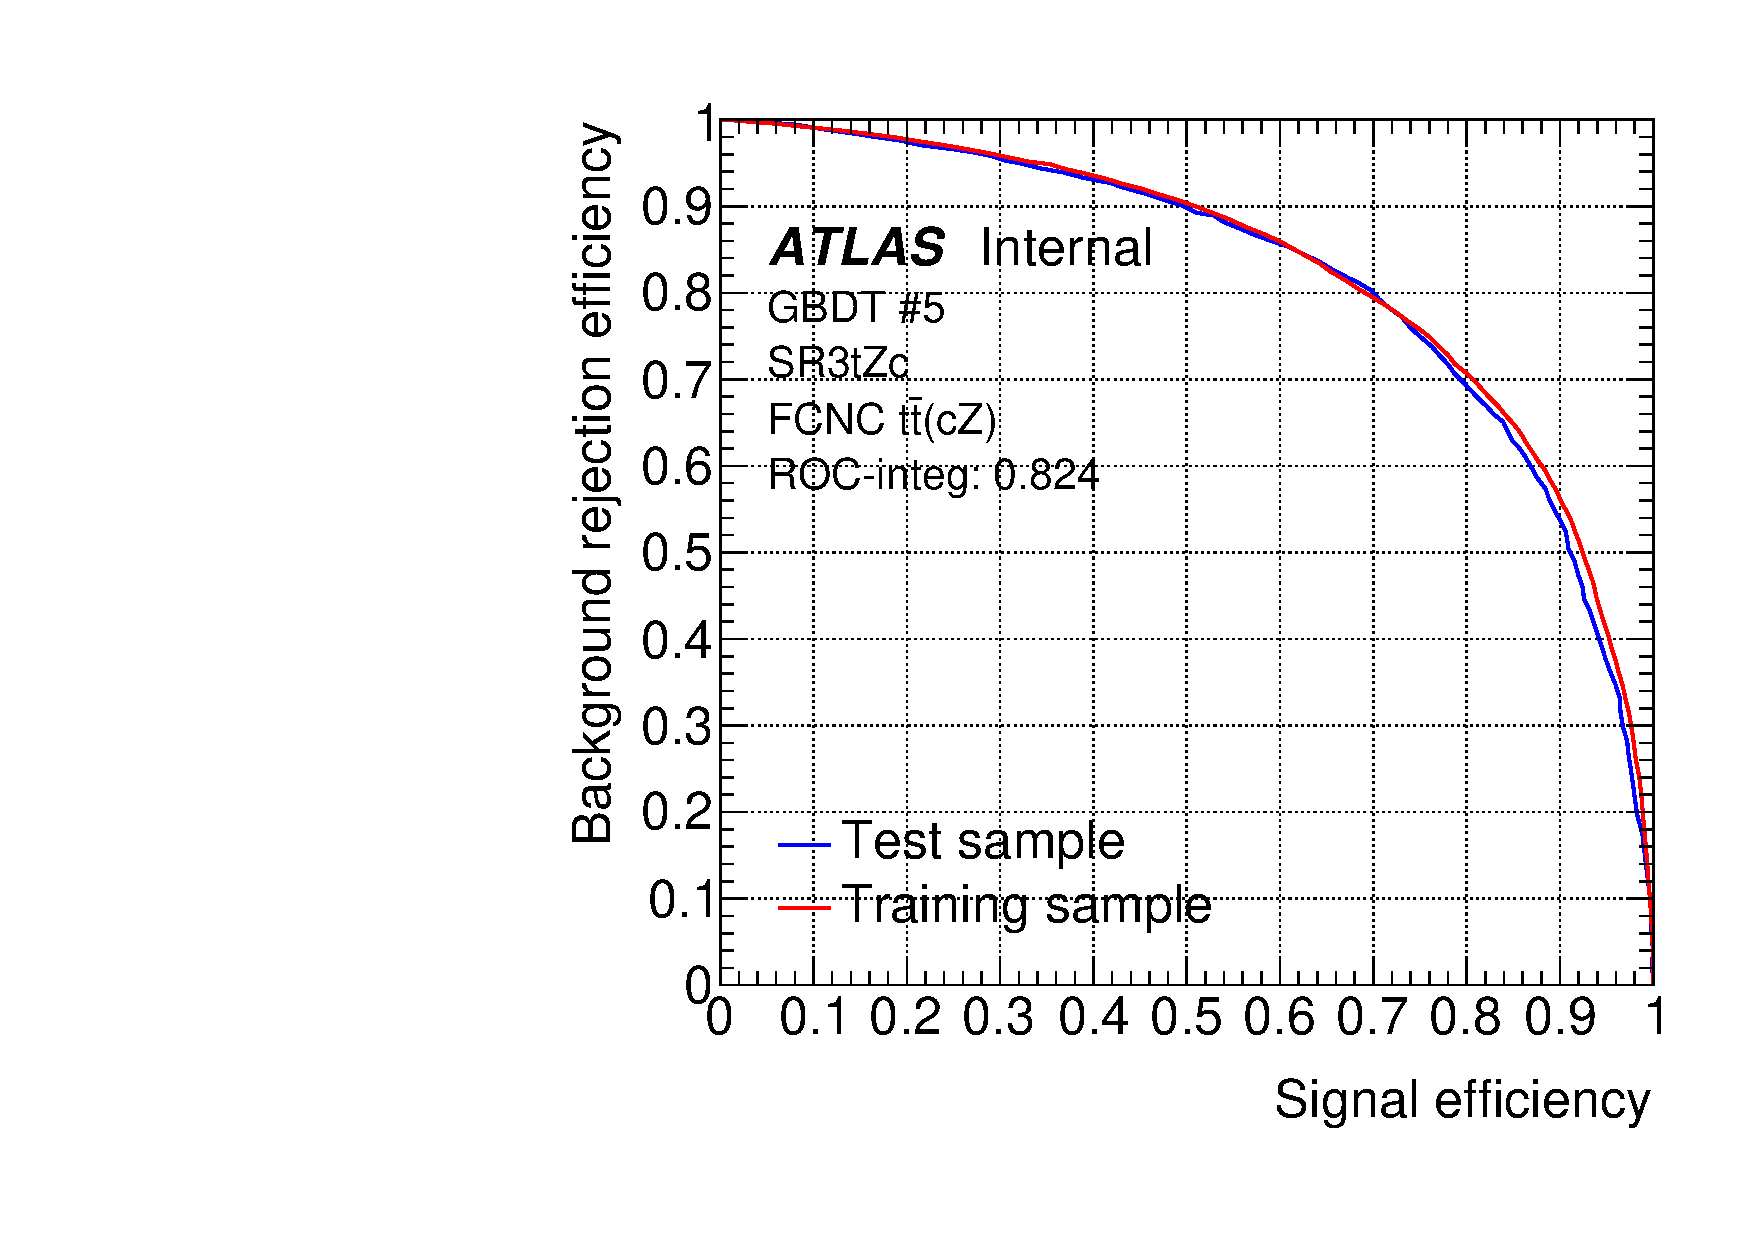
\includegraphics[width=.3\textwidth]{Chapters/CH6/figures/SR3_UsingSMT/BDT/ROC_Fold5}} \\
	\end{tabular}
	\caption{ The ROC curves for each of five GBDTs trained in SR3\tZc to built the \Dthree discriminant. 
		Comparing results between training and test samples.
	}%
	\label{fig:separation:SR3:ROC}
\end{figure}

\begin{figure}[htbp]
	\centering
	\begin{tabular}{ccc}
		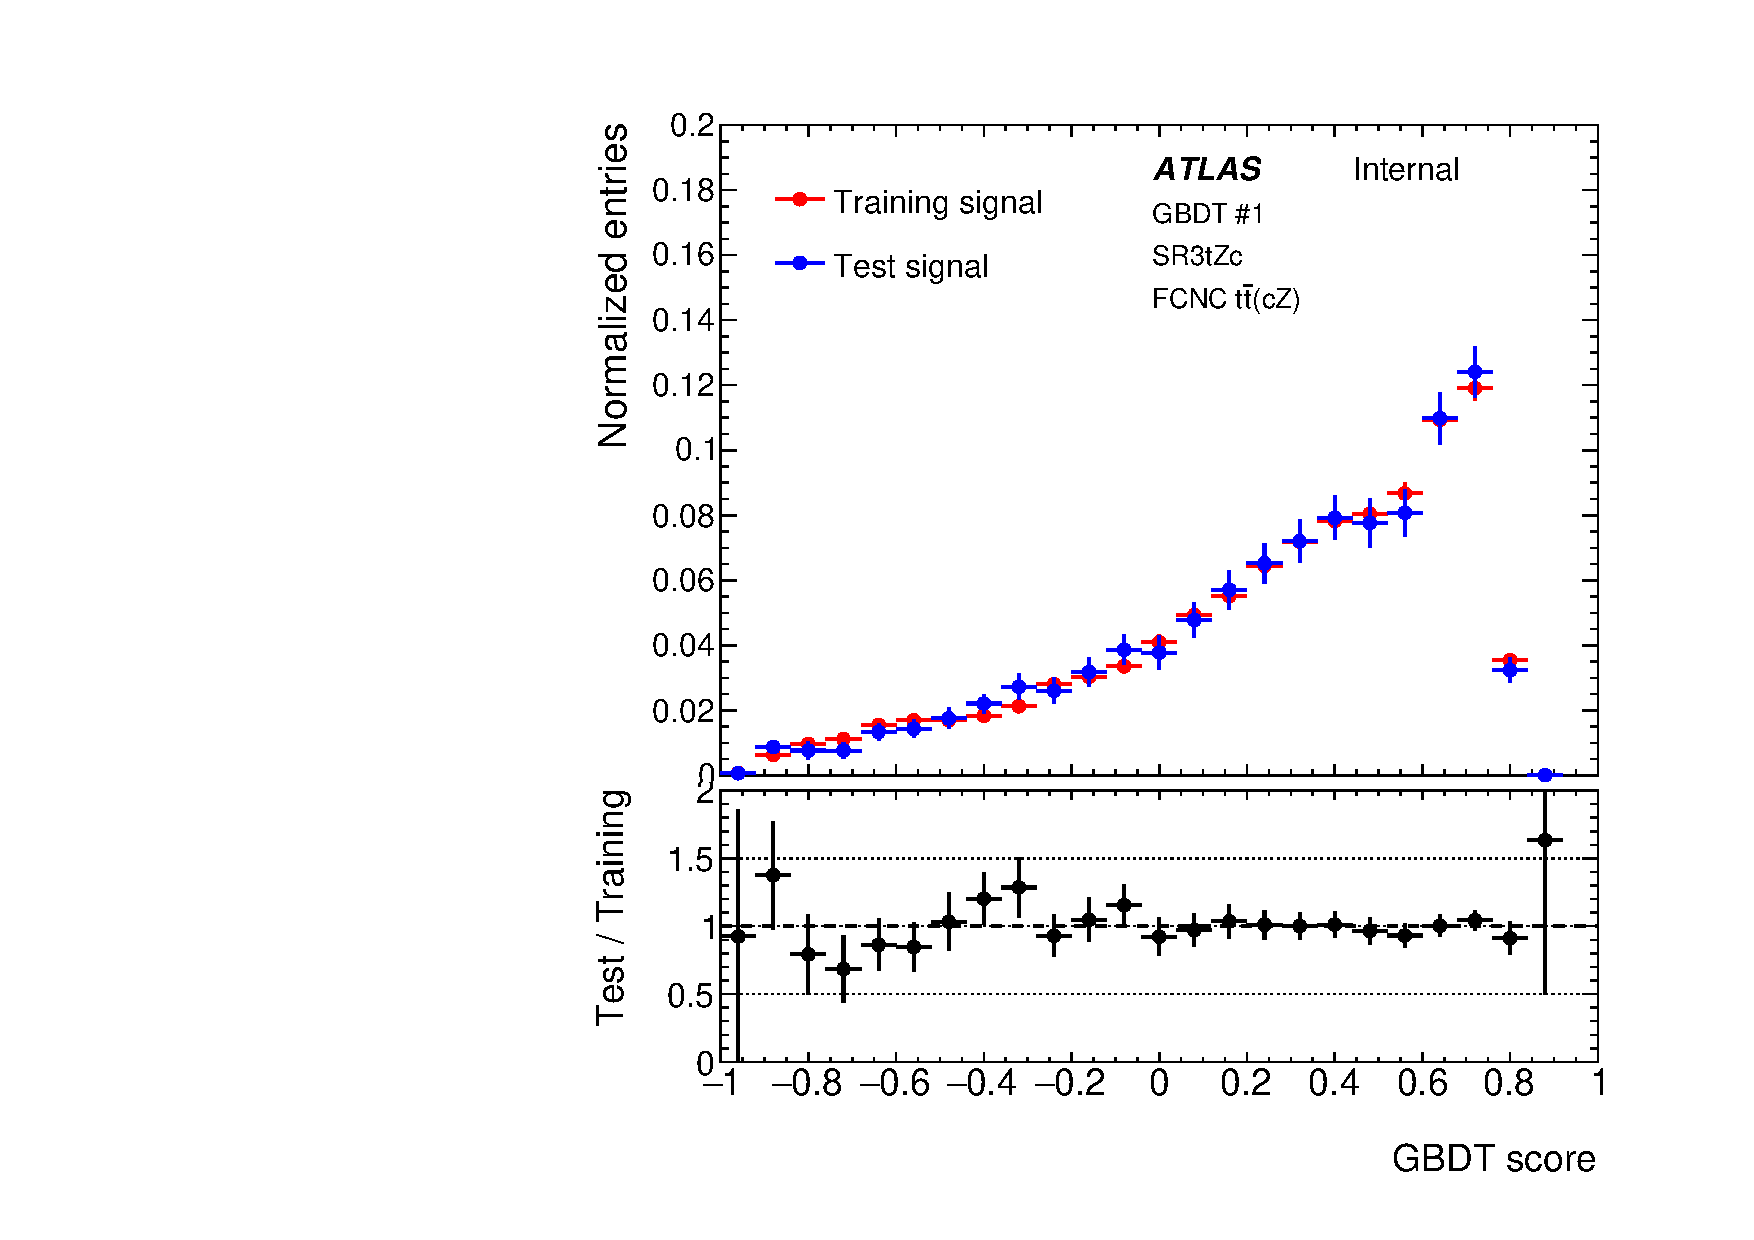
\includegraphics[width=.3\textwidth]{Chapters/CH6/figures/SR3_UsingSMT/BDT/GBDT_signal_Fold1} &
		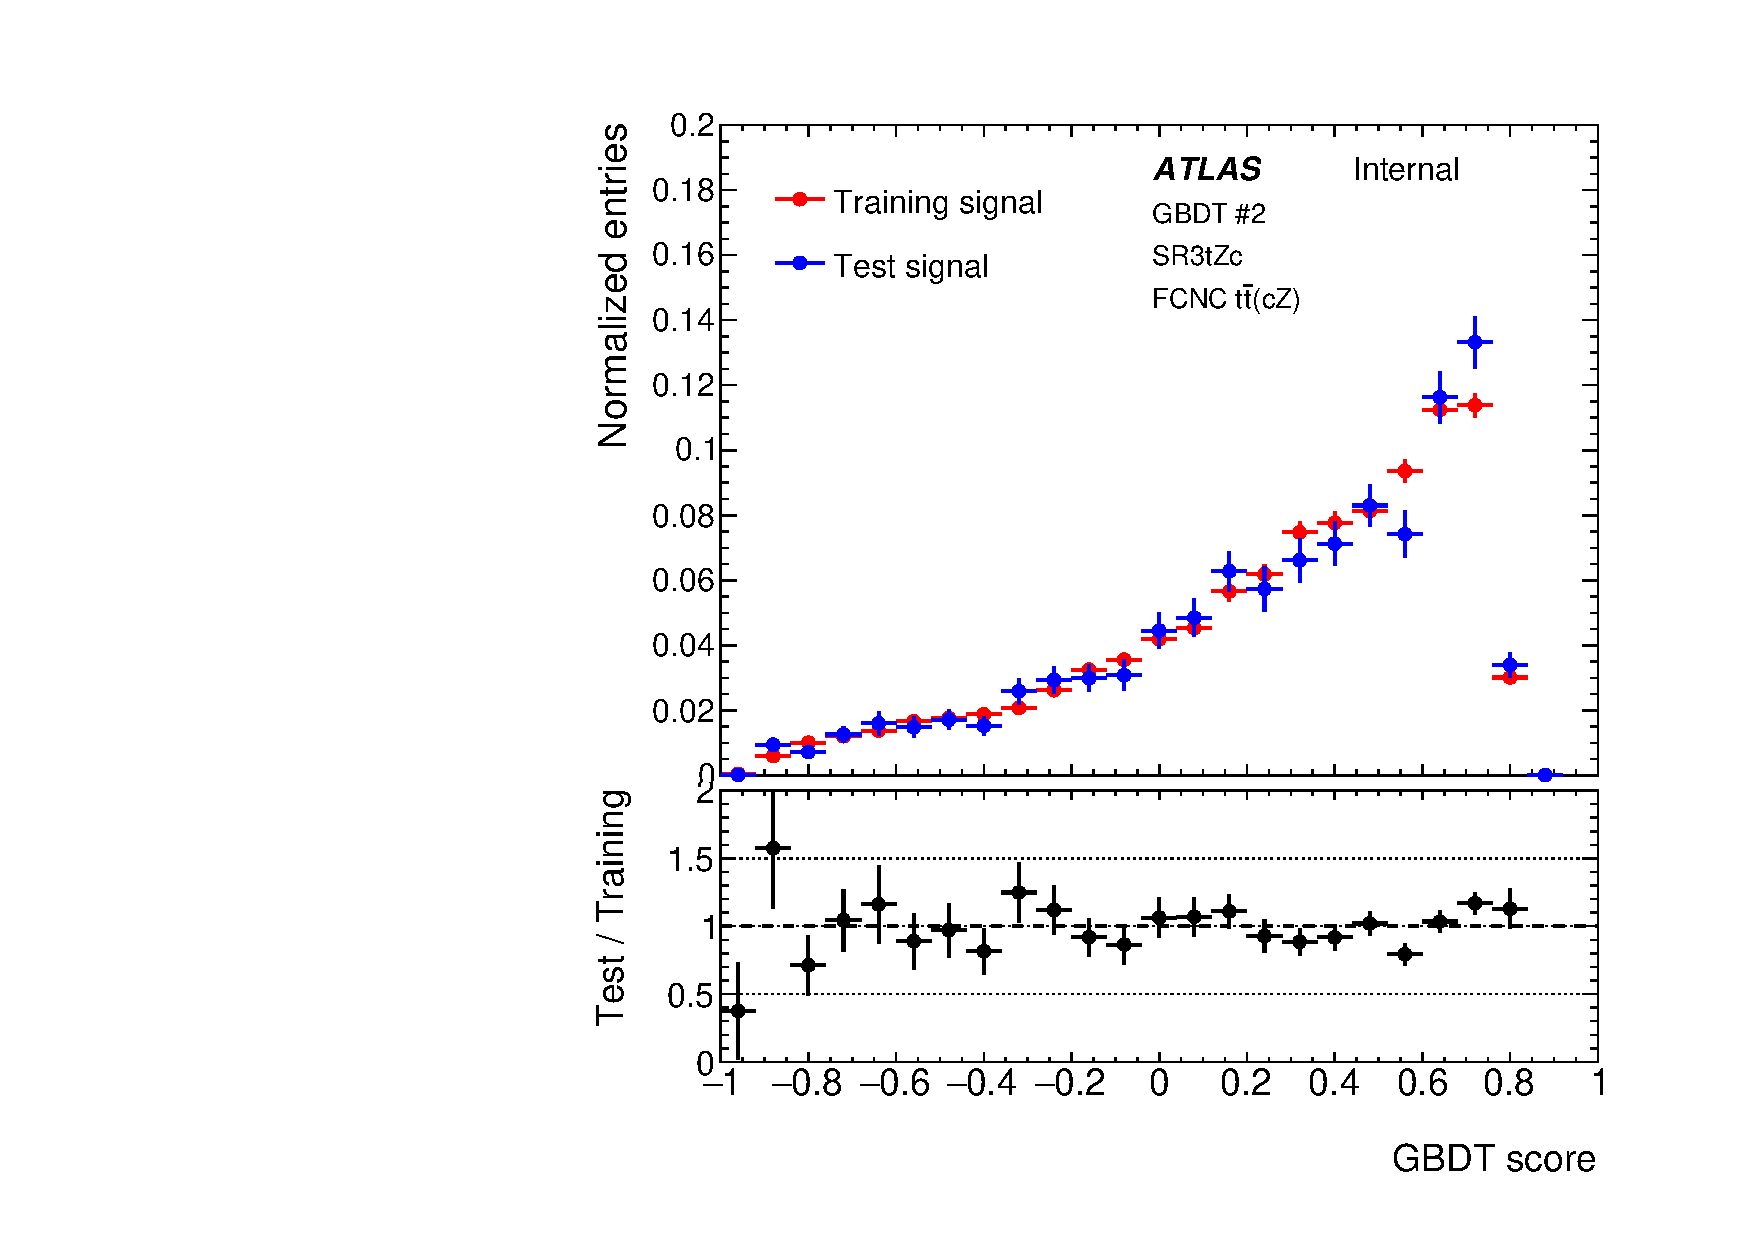
\includegraphics[width=.3\textwidth]{Chapters/CH6/figures/SR3_UsingSMT/BDT/GBDT_signal_Fold2} &
		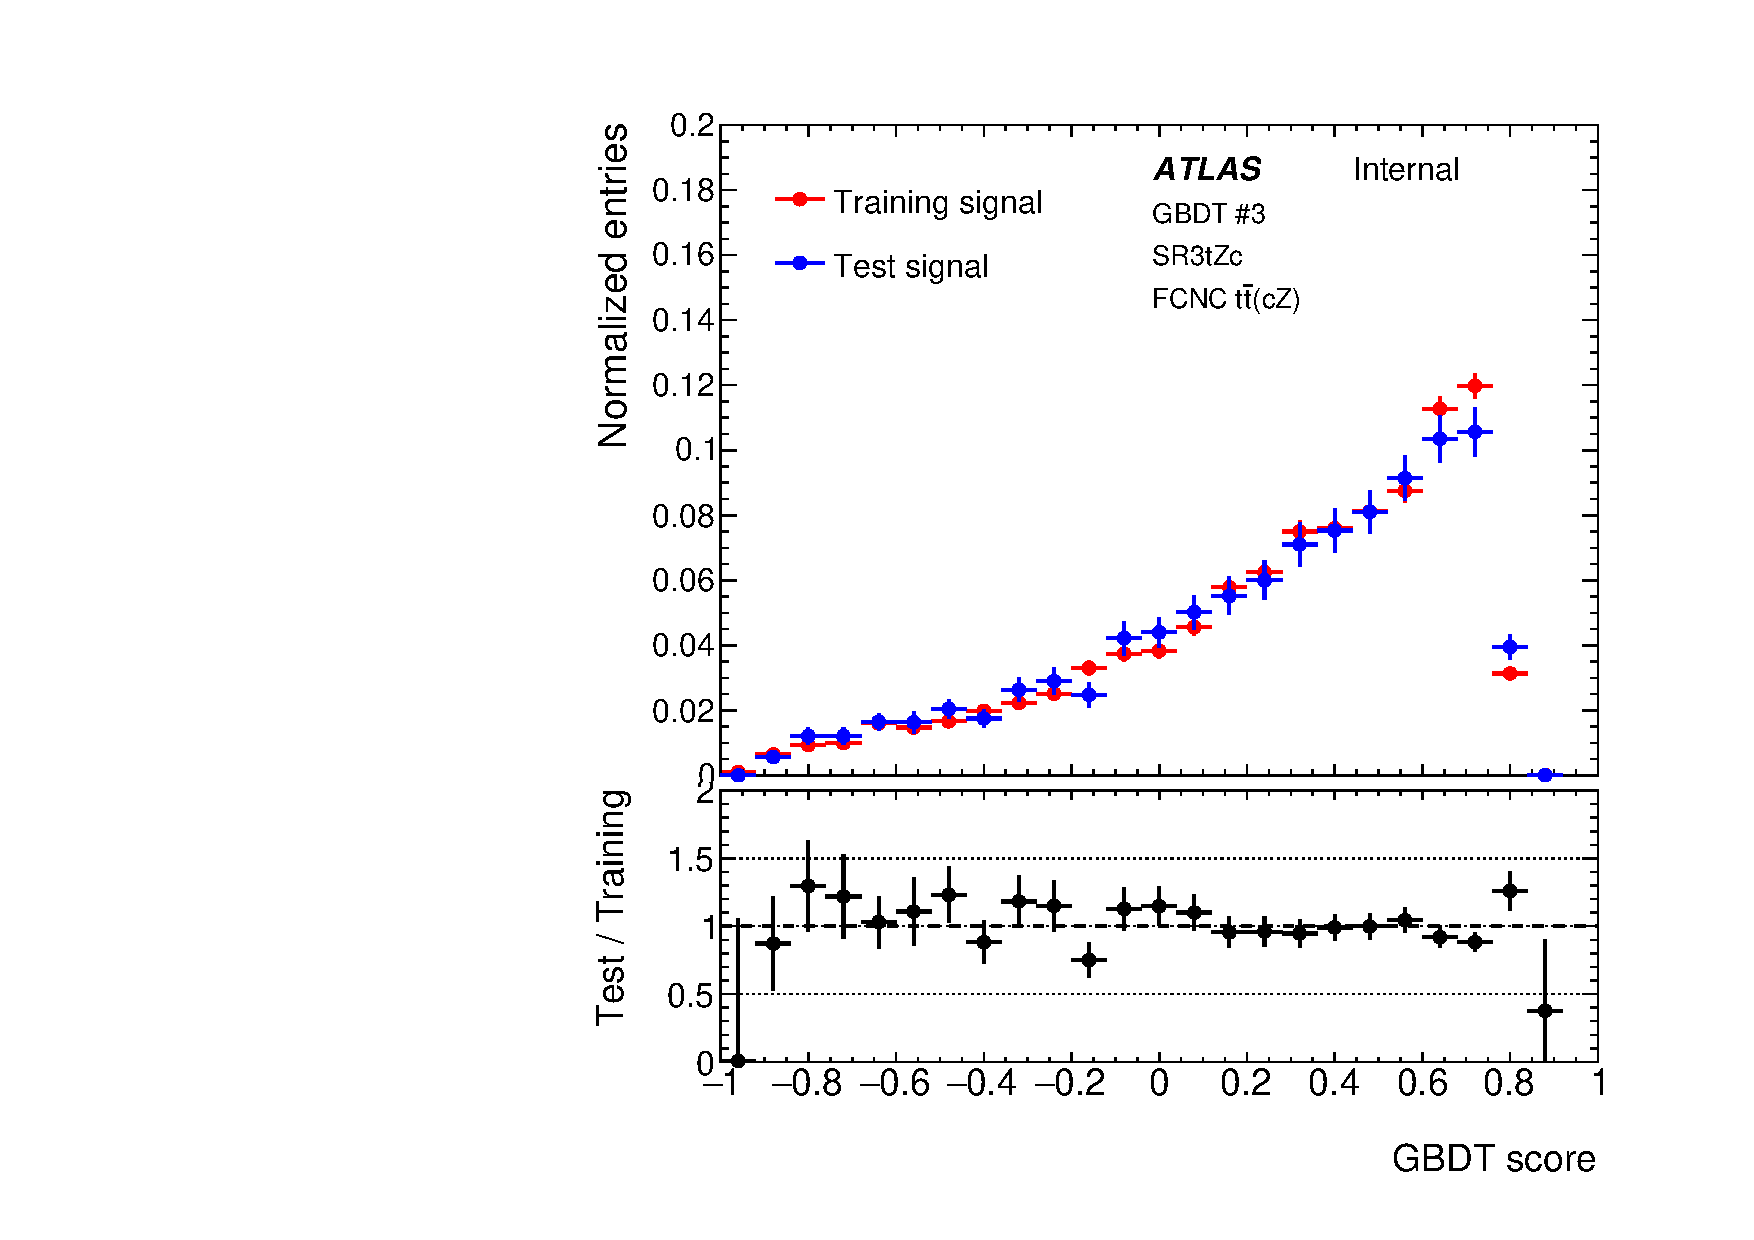
\includegraphics[width=.3\textwidth]{Chapters/CH6/figures/SR3_UsingSMT/BDT/GBDT_signal_Fold3} \\ 
		\multicolumn{3}{c}{
			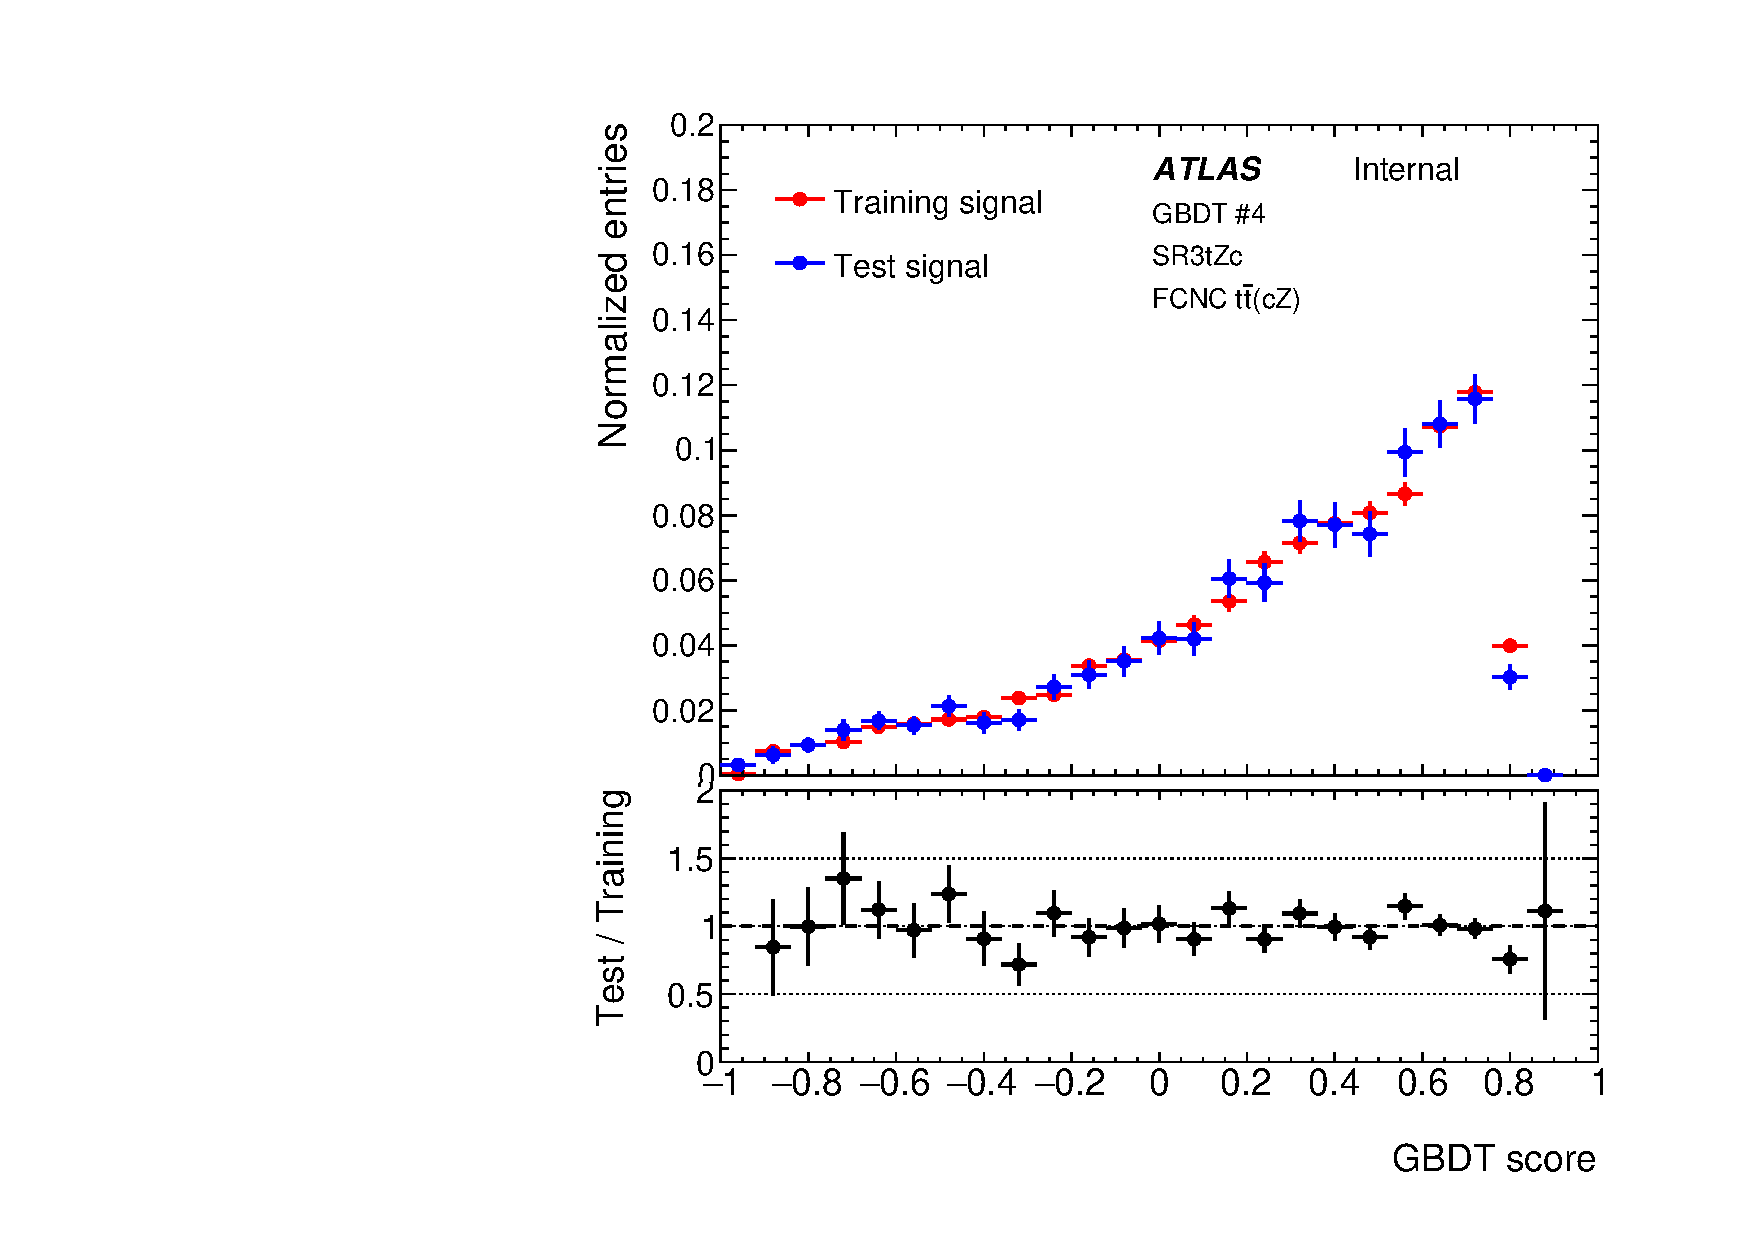
\includegraphics[width=.3\textwidth]{Chapters/CH6/figures/SR3_UsingSMT/BDT/GBDT_signal_Fold4}
			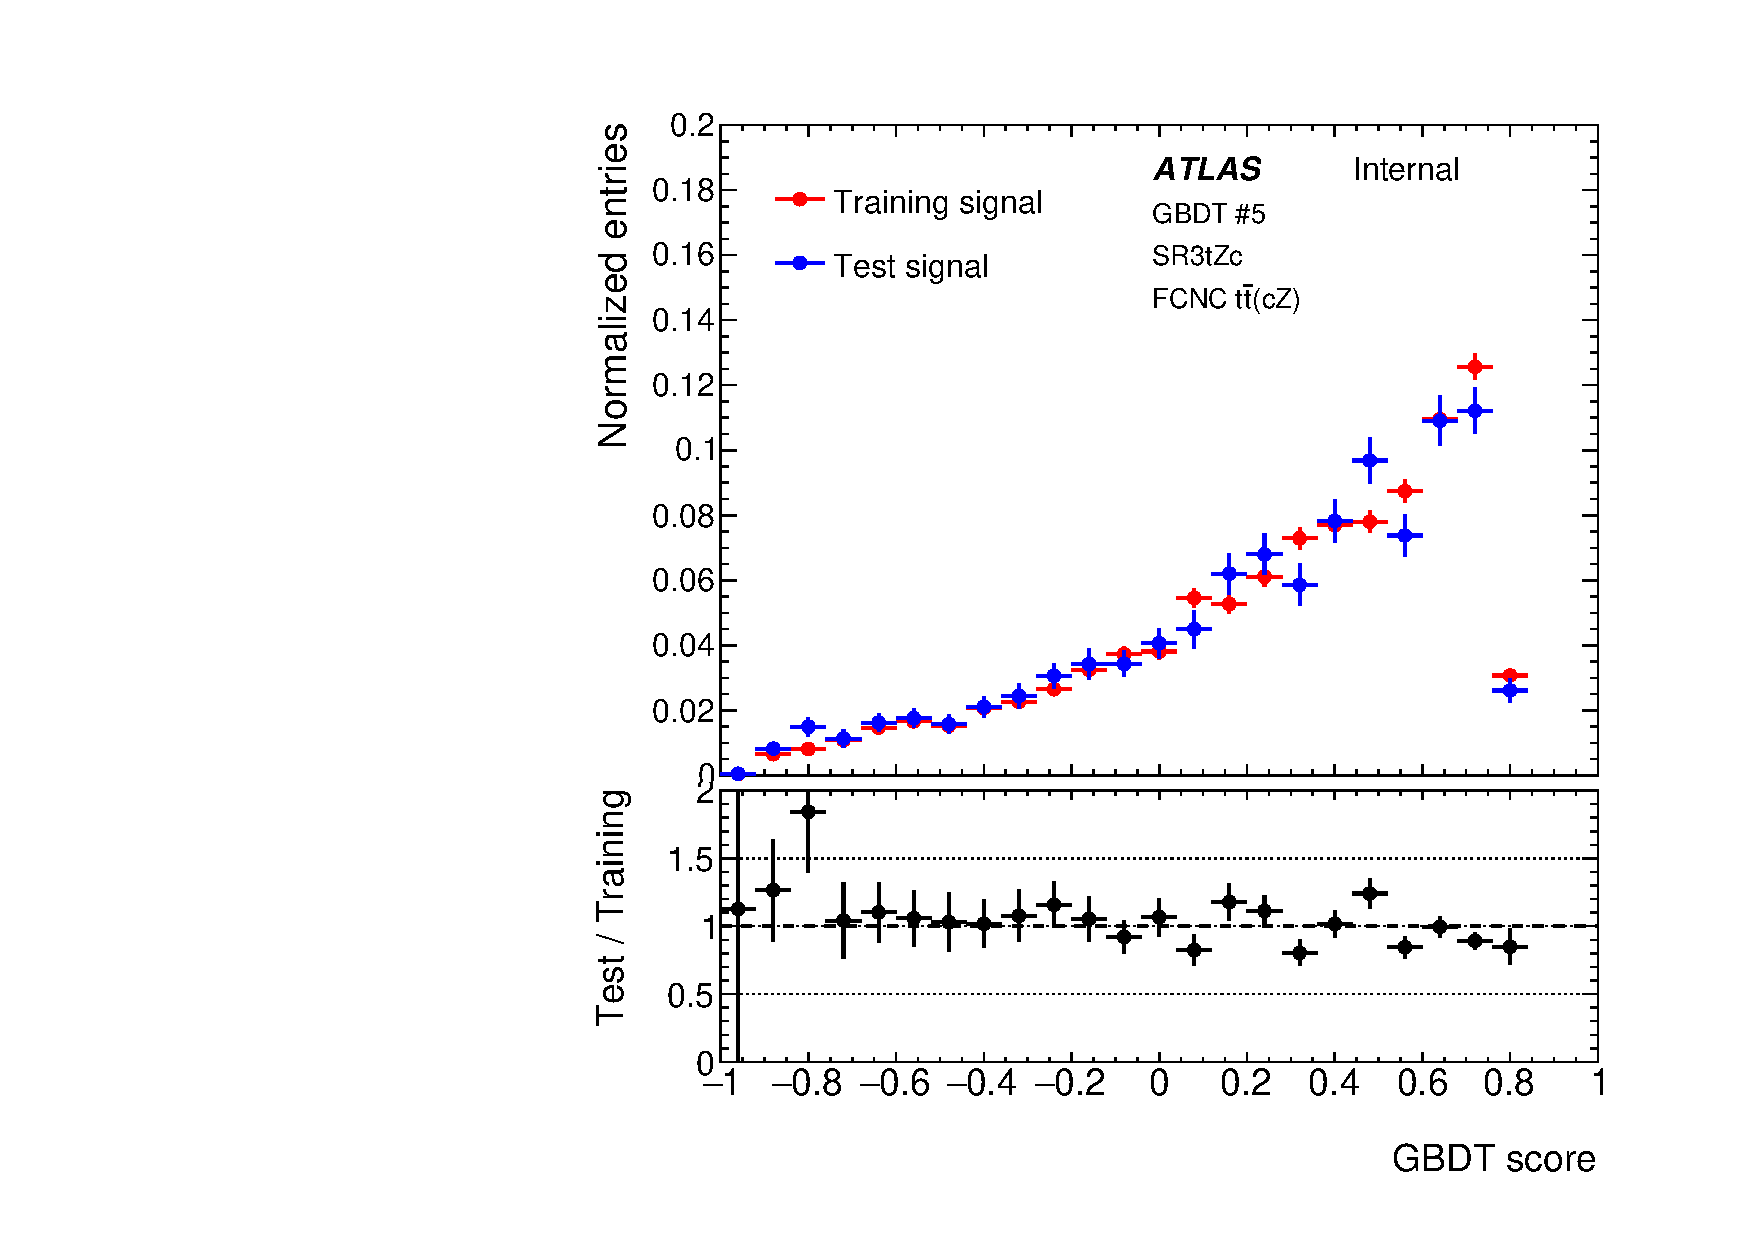
\includegraphics[width=.3\textwidth]{Chapters/CH6/figures/SR3_UsingSMT/BDT/GBDT_signal_Fold5}} \\
	\end{tabular}
	\caption{ The FCNC \tZc \ttbar decay signal GBDT output score distribution for each of five GBDTs trained in SR3\tZc to built the \Dthree discriminant. 
		Comparing results between training and test samples.
	}%
	\label{fig:separation:SR3:GBDTsig}
\end{figure}

\begin{figure}[htbp]
	\centering
	\begin{tabular}{ccc}
		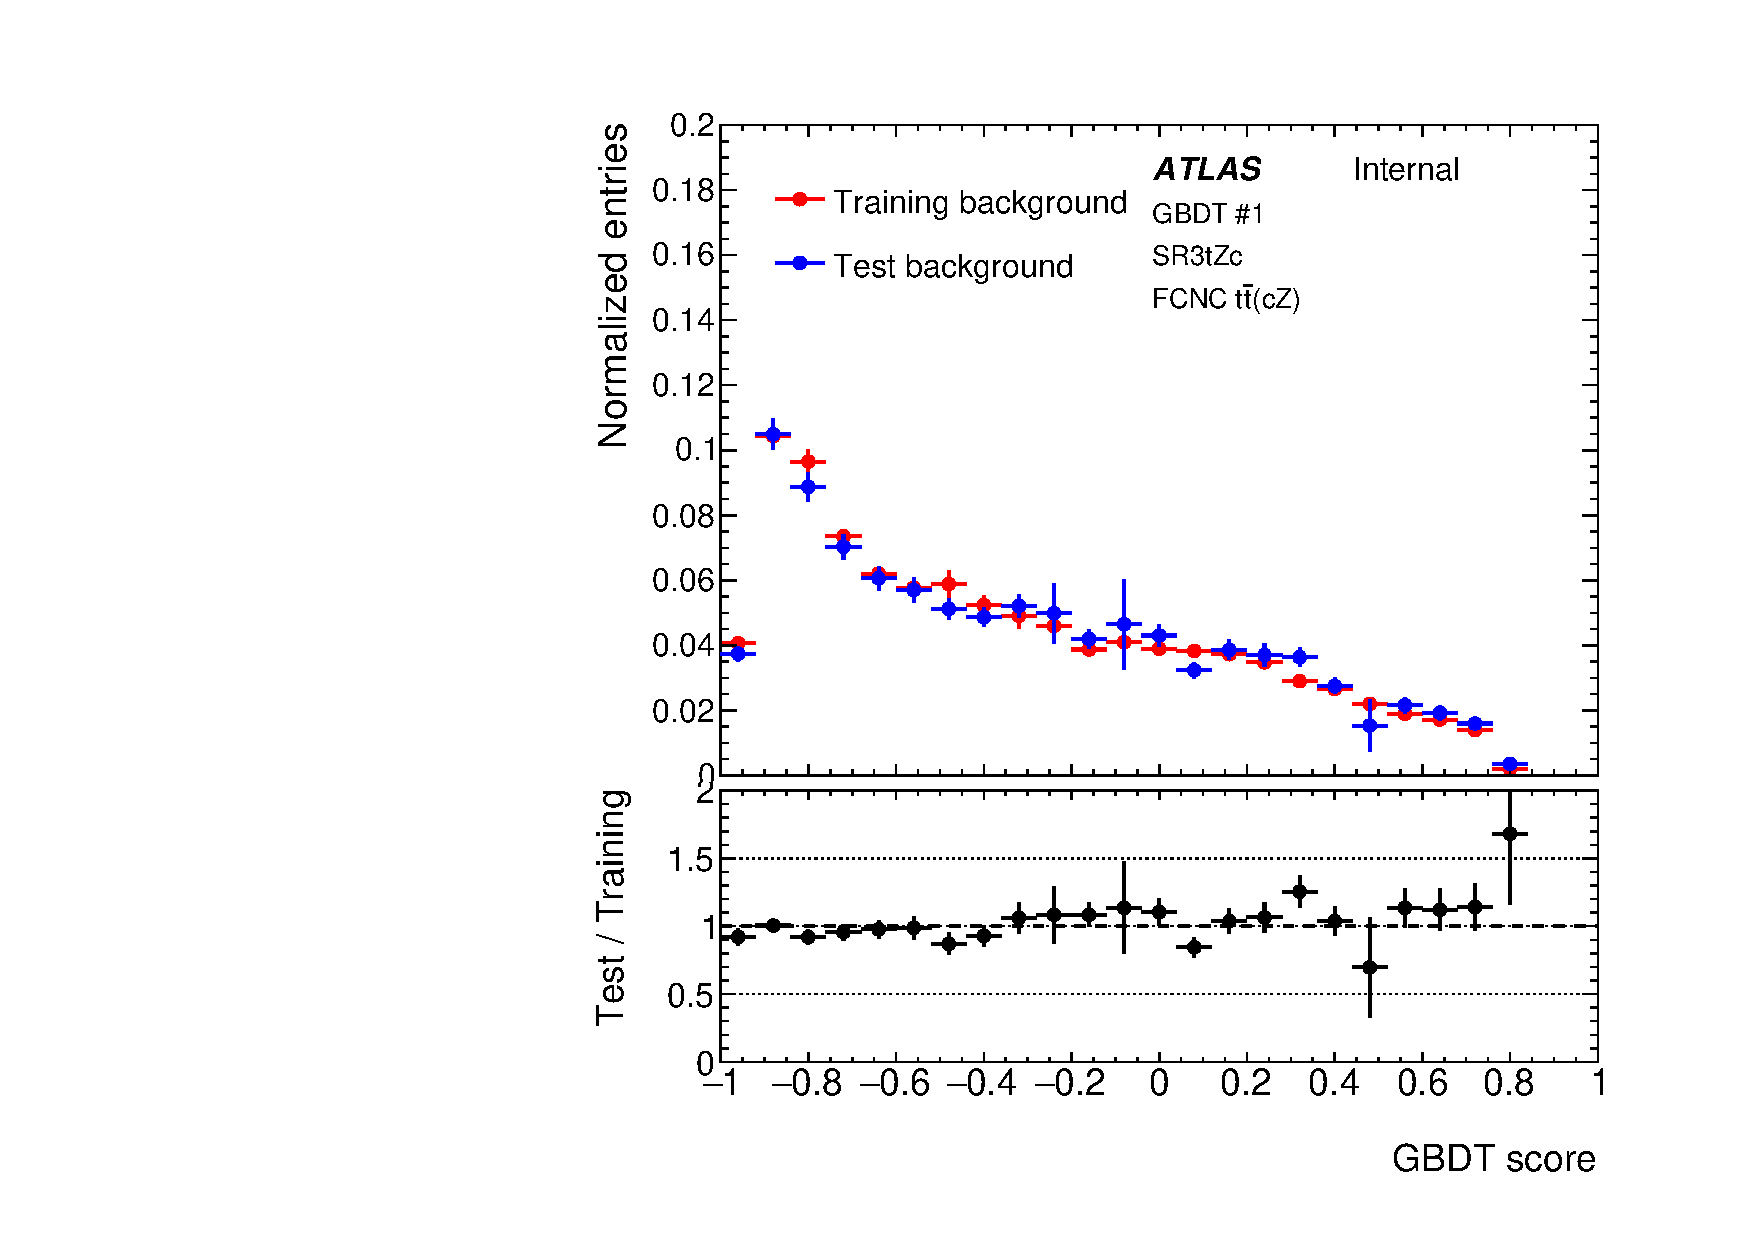
\includegraphics[width=.3\textwidth]{Chapters/CH6/figures/SR3_UsingSMT/BDT/GBDT_background_Fold1} &
		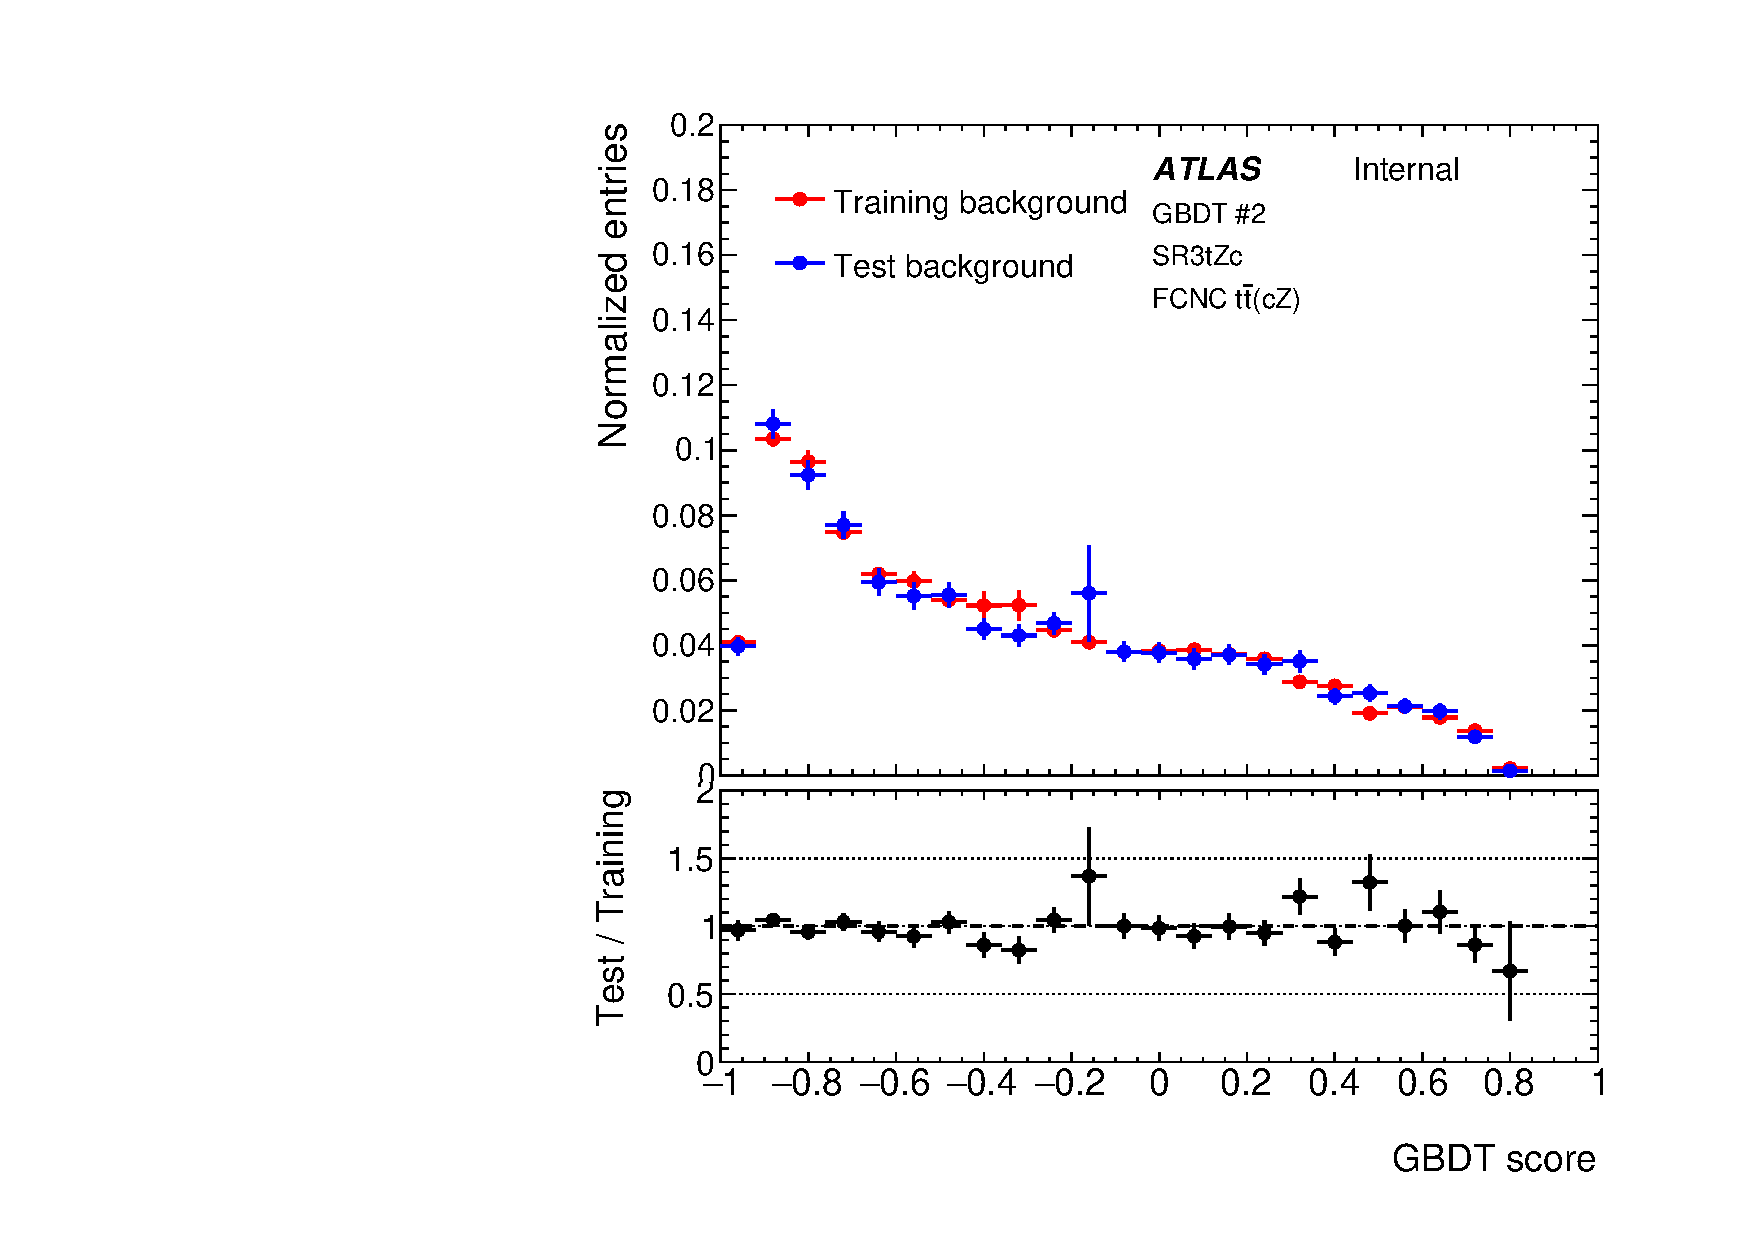
\includegraphics[width=.3\textwidth]{Chapters/CH6/figures/SR3_UsingSMT/BDT/GBDT_background_Fold2} &
		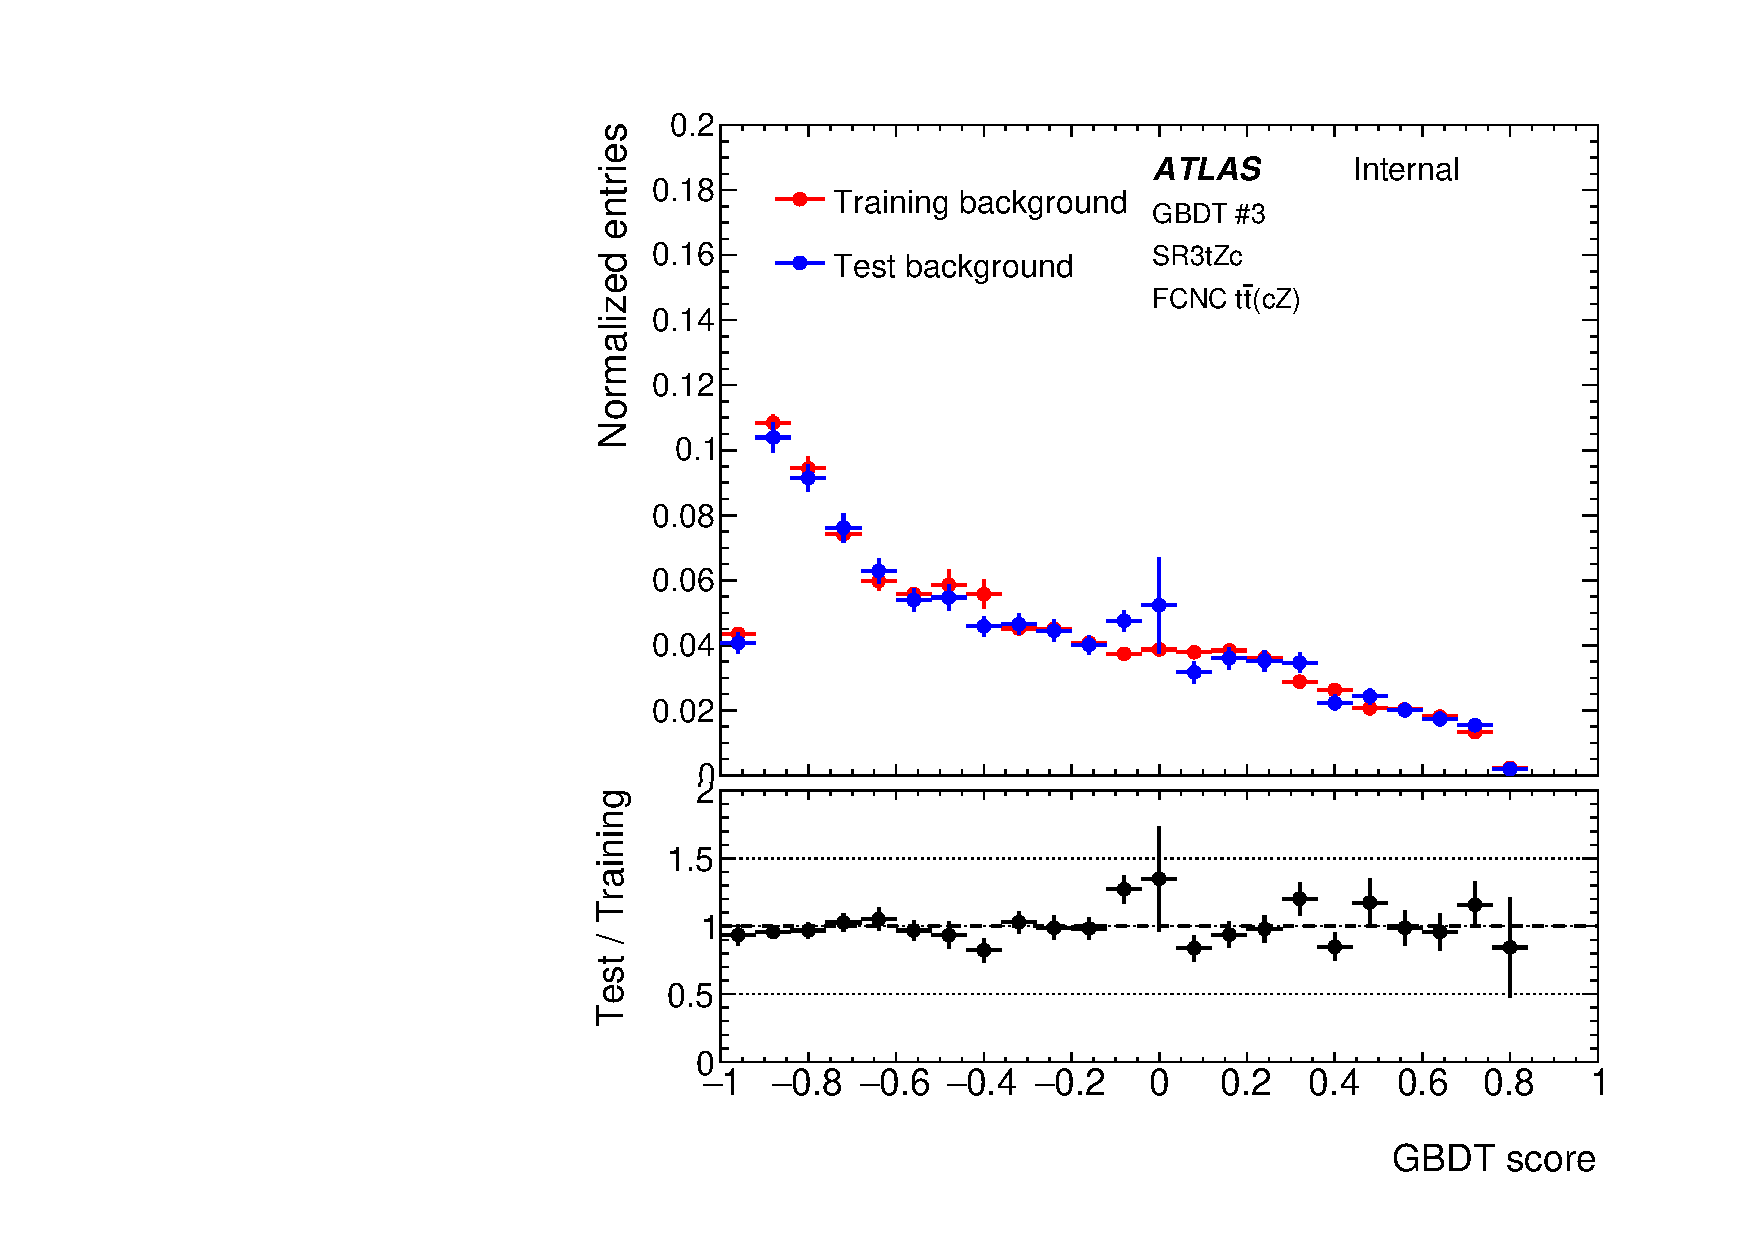
\includegraphics[width=.3\textwidth]{Chapters/CH6/figures/SR3_UsingSMT/BDT/GBDT_background_Fold3} \\ 
		\multicolumn{3}{c}{
		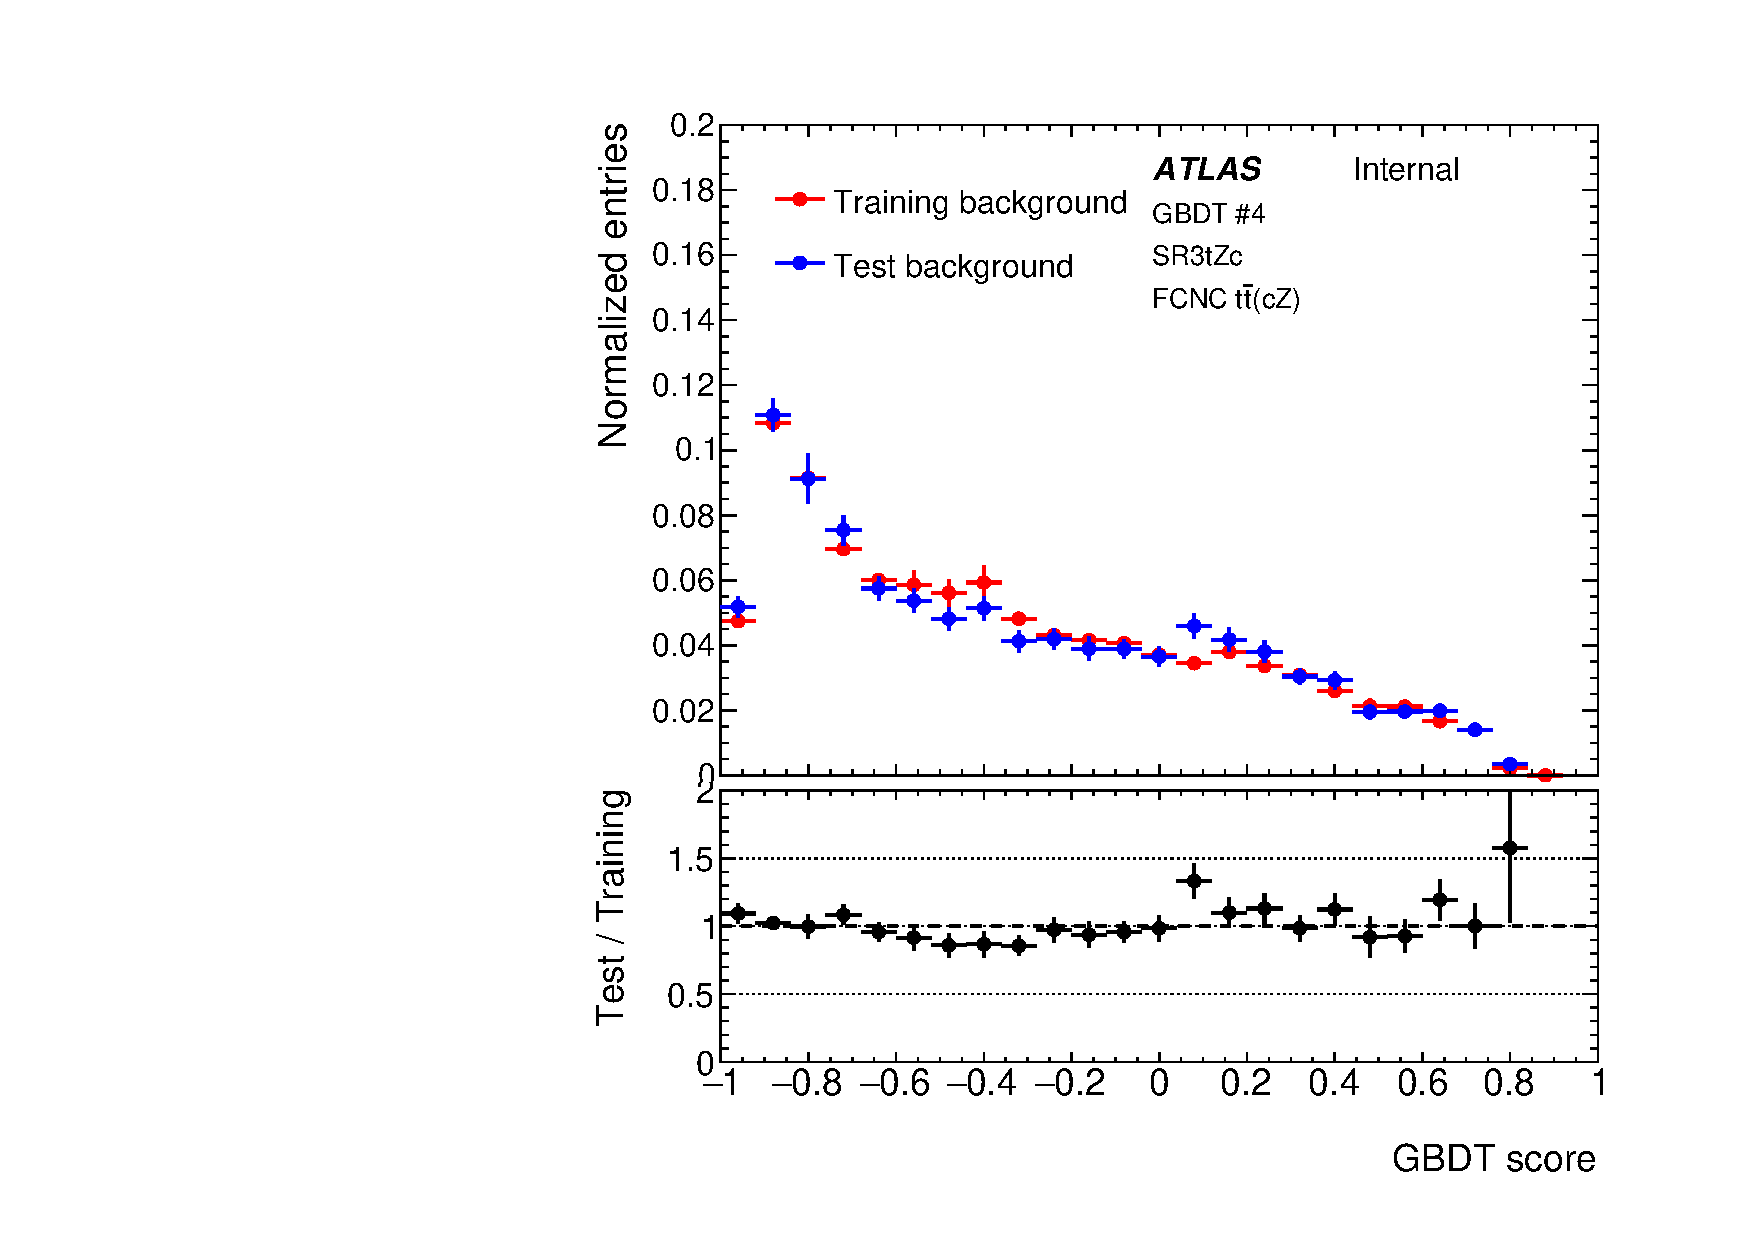
\includegraphics[width=.3\textwidth]{Chapters/CH6/figures/SR3_UsingSMT/BDT/GBDT_background_Fold4}
		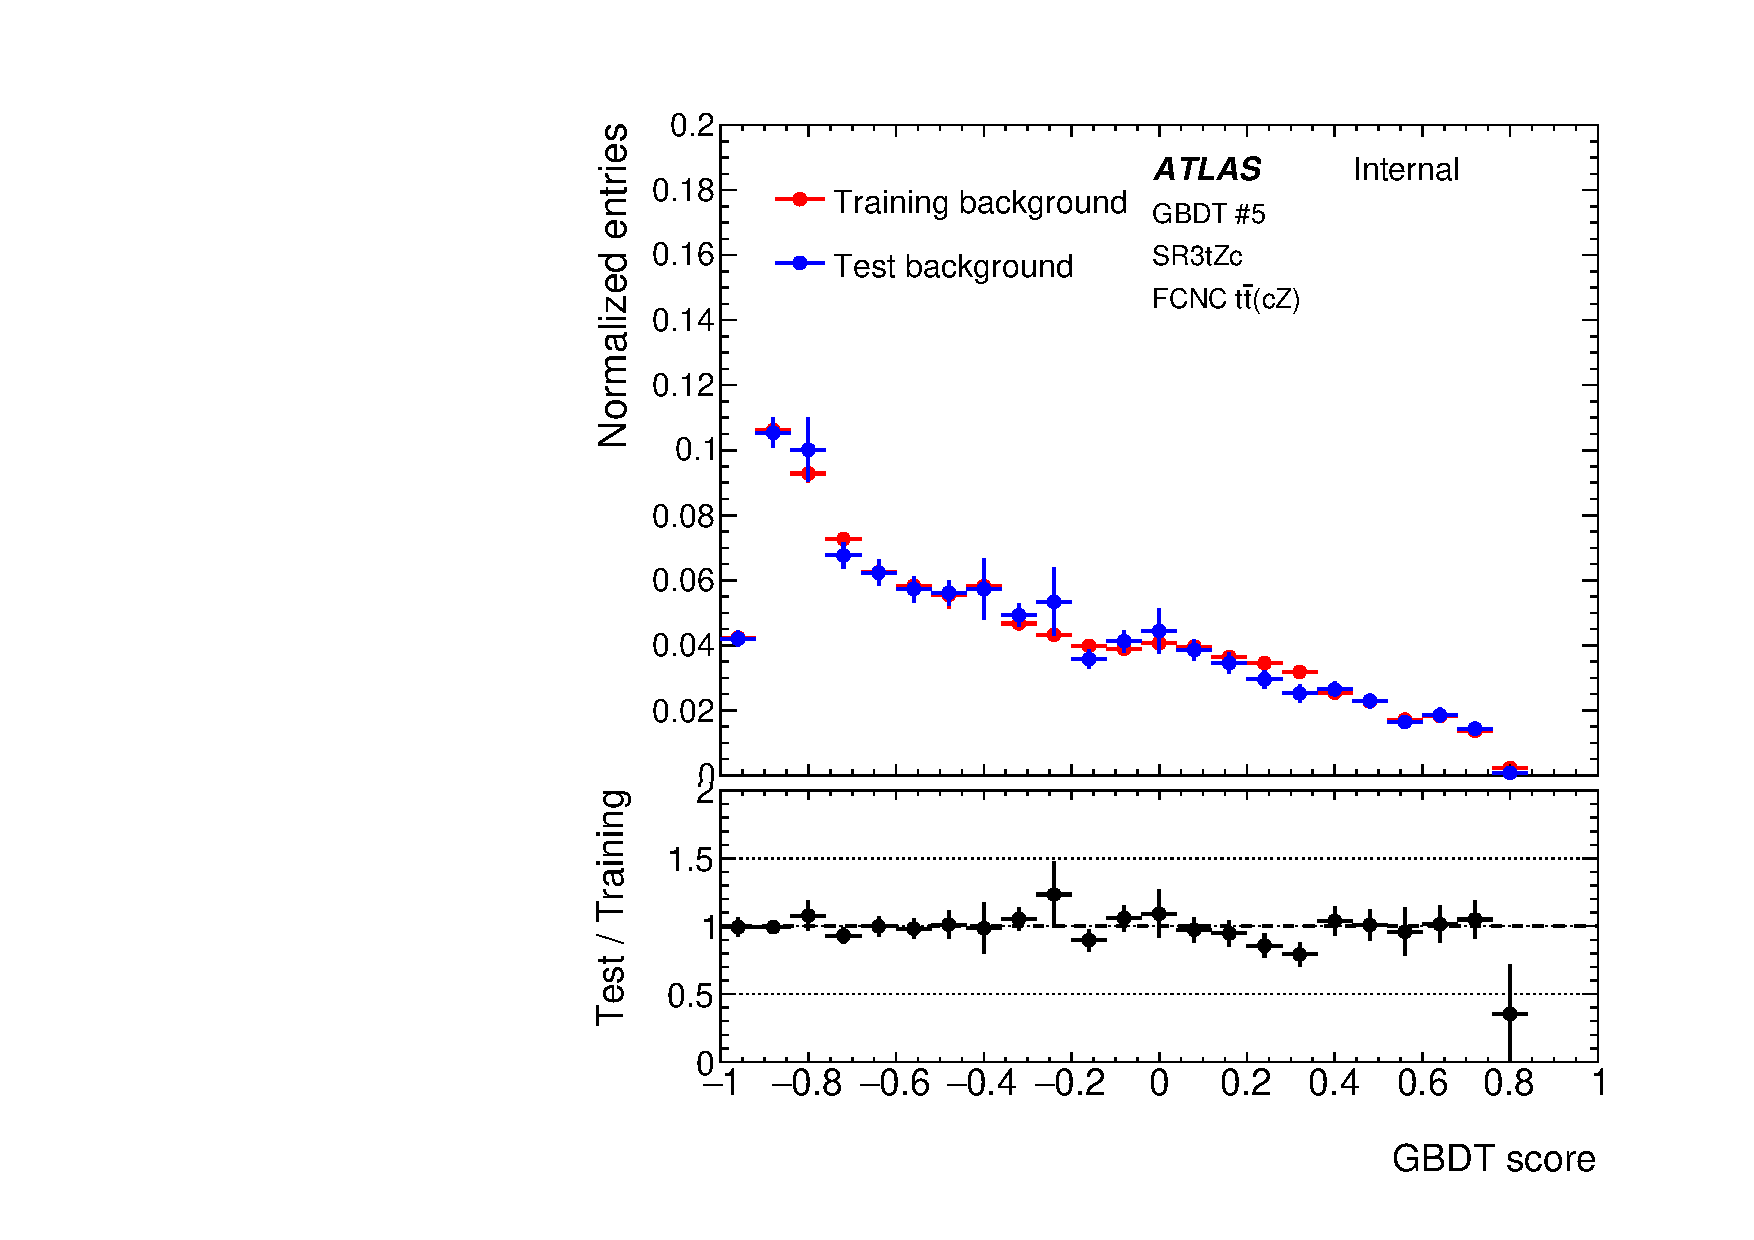
\includegraphics[width=.3\textwidth]{Chapters/CH6/figures/SR3_UsingSMT/BDT/GBDT_background_Fold5}} \\
	\end{tabular}
	\caption{ The background GBDT output score distribution for each of five GBDTs trained in SR3\tZc to built the \Dthree discriminant. 
		Comparing results between training and test samples.
	}%
	\label{fig:separation:SR3:GBDTbkg}
\end{figure}

\begin{figure}[htbp]
	\centering
		\subfigure[]{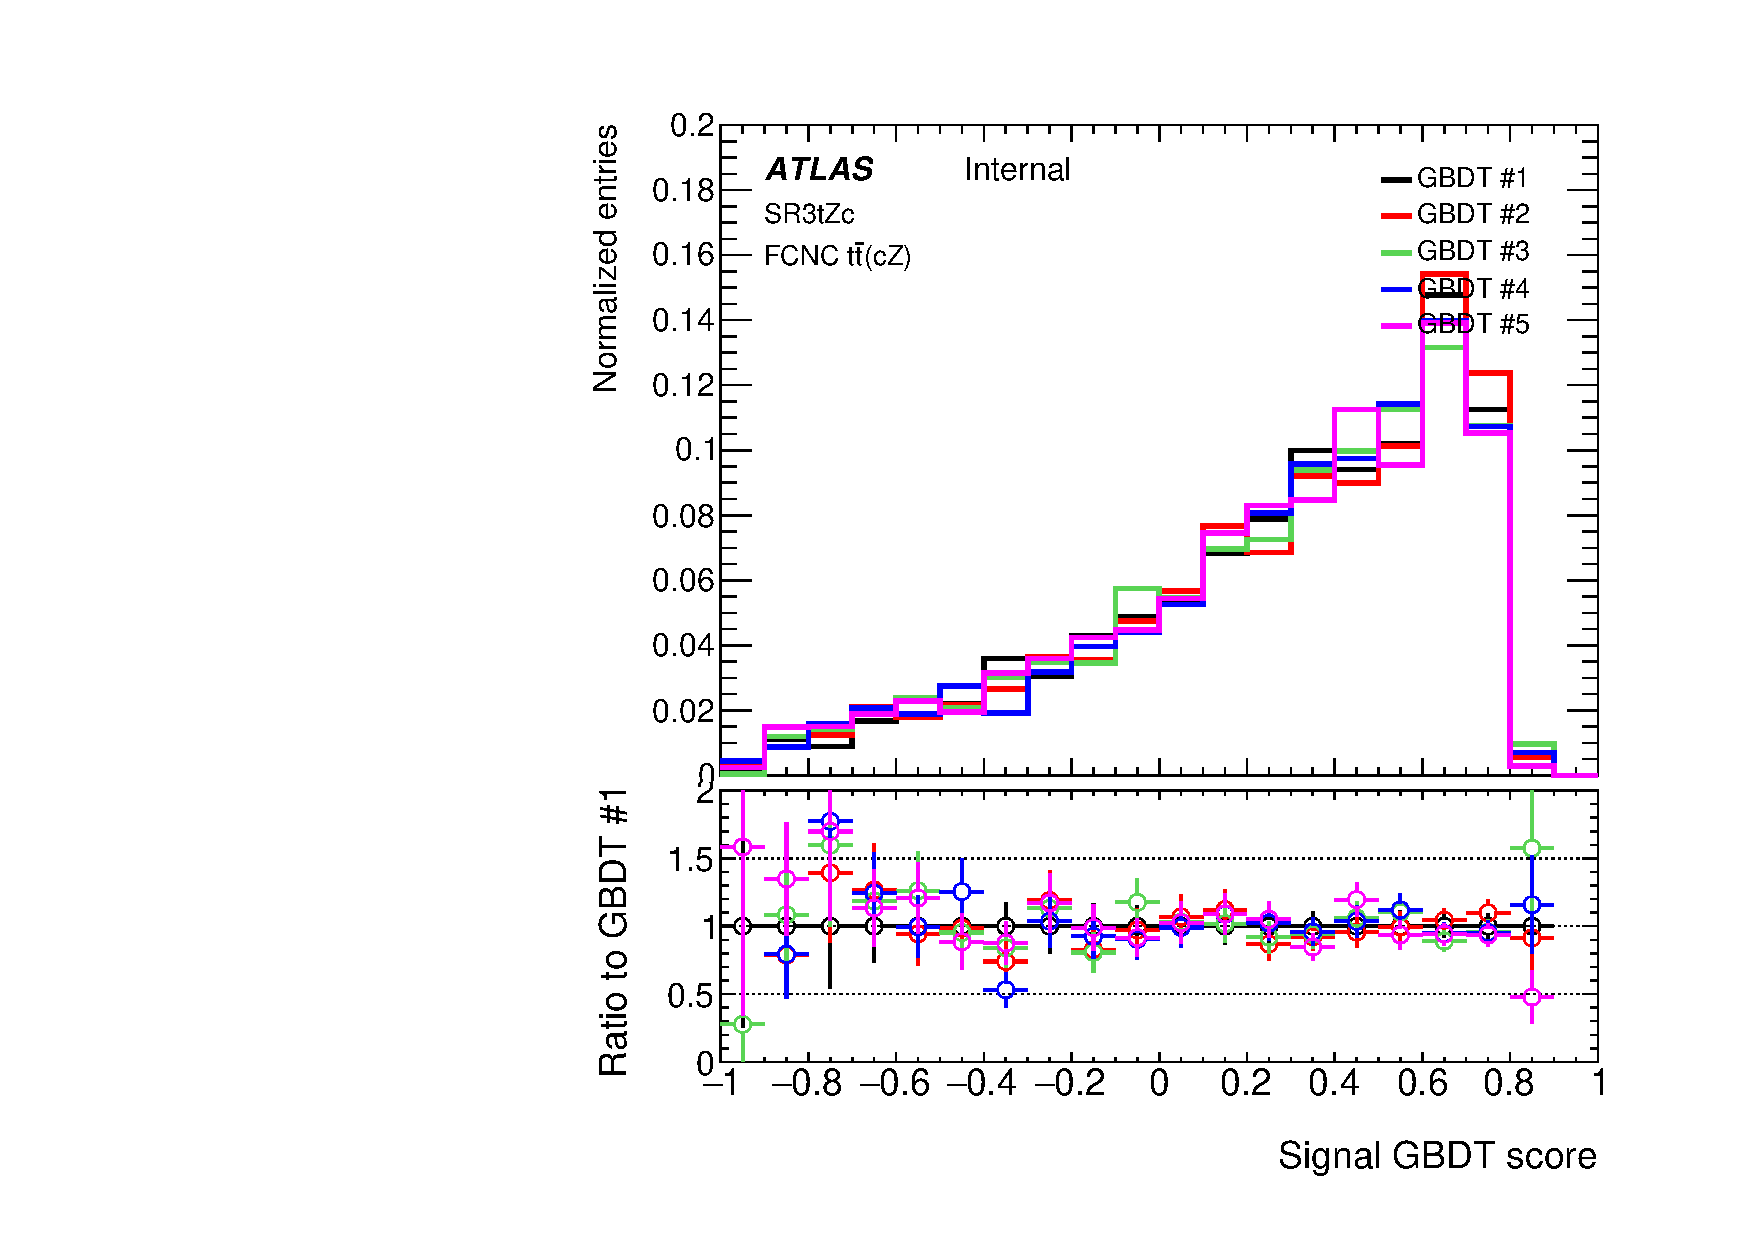
\includegraphics[width=.45\textwidth]{Chapters/CH6/figures/SR3_UsingSMT/BDT/GBDT_signal}\label{subfig:separation:GBDTsig}}\qquad
		\subfigure[]{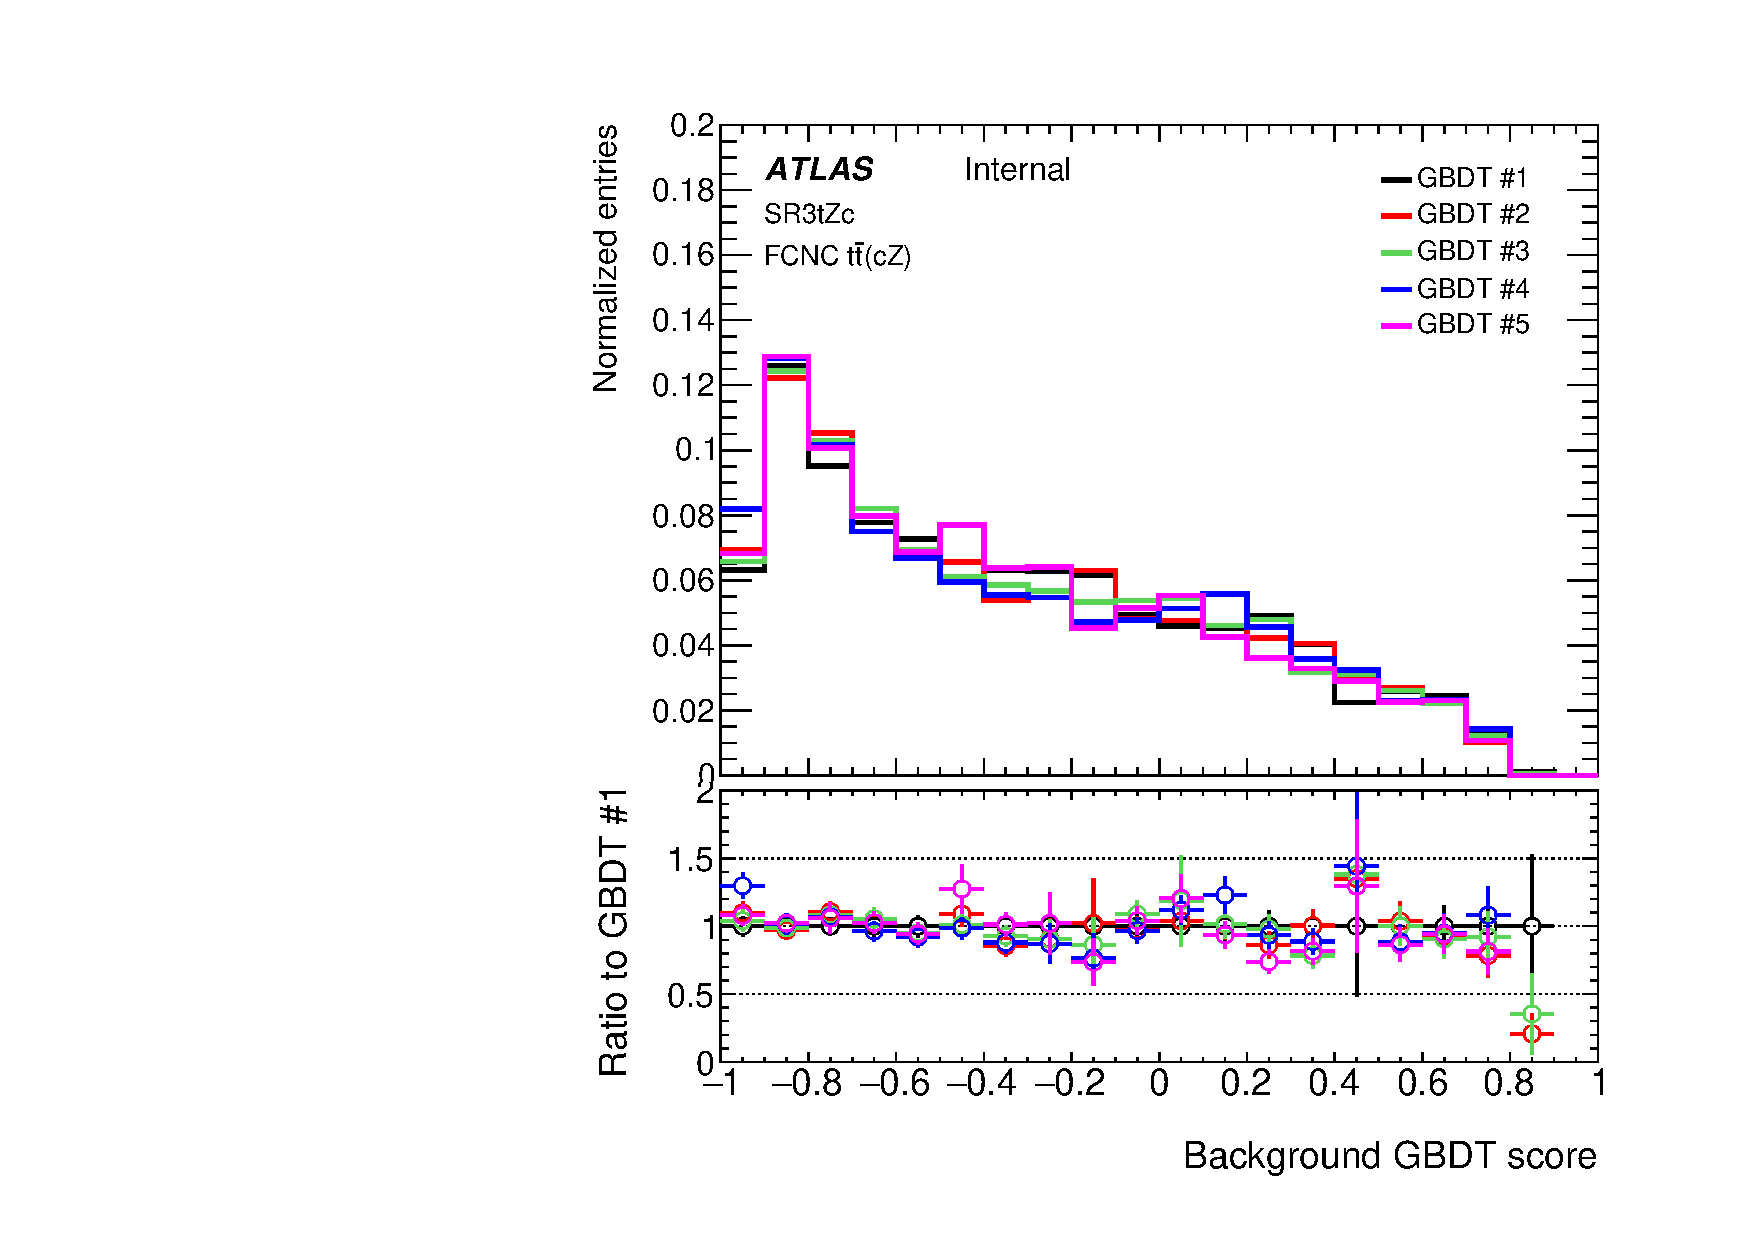
\includegraphics[width=.45\textwidth]{Chapters/CH6/figures/SR3_UsingSMT/BDT/GBDT_background}\label{subfig:separation:GBDTbkg}}
	\caption{ The GBDT output score distributions for \subref{subfig:separation:GBDTsig} signal events and \subref{subfig:separation:GBDTbkg} background events, in the test samples.
		Trained five GBDTs are compared in each signal region. 
	}%
	\label{fig:separation:GBDT}
\end{figure}

\clearpage
\section {The alternative c-tagger $\mathrm{DL1r_{c}}$}
\label{sec:other_selection}
The alternative c-tagger $\mathrm{DL1r_{c}}$ (see \Cref{sec:object:cjet}) has been investigated for SR3\tZc as an alternative to SMT, already discussed in \Cref{sec:sel:sr3}.\\
The requirements in this region are the following:
\begin{itemize}
	\item At least two jets satisfying the requirements described in \Cref{sec:object:jet}. 
	\item Exactly one \Pqb-jet satisfying the requirements in \Cref{sec:object:bjet}. 
	\item At least one c-jets satisfying the requirements described in \Cref{sec:object:cjet}.
	\item No requirements on the masses of both the FCNC and the SM top-quark candidates are applied. 
\end{itemize}
The event yield for  for this selection is shown in Table~\ref{tab:yields:sr3_dl1rc}.
\begin{table}[!h]
	\centering
	\small
	\begin{tabular}{|l|l|}
		\hline
		\textbf{Sample}                  			 & \textbf{Total yield}     \\
		\hline
		ZZ+LF                 & 0.71 $\pm$ 0.07          \\   
		ZZ+HF                 & 5.31 $\pm$ 0.13         \\   
		WZ+LF                  & 2.18 $\pm$ 0.12         \\   
		WZ+HF                  & 25.02 $\pm$ 0.39         \\   
		VV (2l)                 					  & 0.05 $\pm$ 0.04                             \\   
		WtZ                       					  & 12.39 $\pm$ 0.49                                \\   
		$t\bar{t}W$             					  & 2.04 $\pm$ 0.12                             \\   
		$t\bar{t}Z$ (2l)       					      & 0.02 $\pm$ 0.02                             \\   
	    $t\bar{t}Z$           &69.49 $\pm$ 0.61   \\   
		Wt                      					  & 0.00 $\pm$ 0.00                           \\   
		tZ                      					  & 13.82 $\pm$ 0.28                            \\     
		$t\bar{t}$             						  & 3.66 $\pm$ 0.37                            \\   
		Z+jets                 						  & 1.32 $\pm$ 0.58                            \\   
		4 tops                 						  & 0.09 $\pm$ 0.01                           \\   
		3 tops                 						  & 0.02 $\pm$ 0.00                           \\   
		VVV                     					  & 0.22 $\pm$ 0.02                           \\   
		VH                      					  & 0.00 $\pm$ 0.00                           \\   
		$t\bar{t}H$             					  & 2.63 $\pm$ 0.05                           \\   
		$t\bar{t}WW$          					      & 0.16 $\pm$ 0.04                           \\   
		\hline                                                                    
		Total bkg.              					  &  139.13 $\pm$ 1.17                          \\       
		\hline                                                                     
		FCNC $t\bar{t}$(cZ)   					      &  21.94 $\pm$ 0.39                \\
		FCNC (c)tZ              				      &  1.21 $\pm$ 0.03                          \\
%		\hline                                                                    
%		$S/\sqrt{B}$ (ctZ)      					  &  1.96 $\pm$ 0.02                      \\
		\hline
	\end{tabular}
	\caption{Total event yield for the SR3\tZc selection using the c-tagger $\mathrm{DL1r_{c}}$.}
\label{tab:yields:sr3_dl1rc}
\end{table}  
\newline \noindent Comparing the two event yield in Table~\ref{tab:yields:sr3} with Table~\ref{tab:yields:sr3_dl1rc} is possible to see that using \DLrc the number of signal events is significantly larger than using SMT since the semi-leptonic decay of heavy hadrons is limited by the branching ratio ($\simeq$ 20\%).
However, taking into account the SMT selection with only one b-jet, it is also possible to see that SMT has a better discrimination of backgrounds manly due to a better light-rejection.\\
To choose the best selection, one can compare the values of \ssplusb for each bin of the GBDT discriminant as can bee seen in Table~\ref{tab:yields:sr3_smt_bdt} for the SMT selection, in Table~\ref{tab:yields:sr3_dl1rc_bdt} for \DLrc selection, and Figure~\ref{fig:yields:sr3_bdt}.\\
For the \DLrc selection, in the last three bins of the GBDT discriminant, there are
12.3 events of signal and 9.3 events of background 
which corresponds to more signal events and 10\% background events of the whole SR3\tZc with SMT. The GBDT output for SMT is presented in \Cref{sec:separation} while for \DLrc it will be presented in \Cref{sec:separation_all}.
\begin{figure}[!htbp]
	\centering
	\subfigure[SMT selection]{
		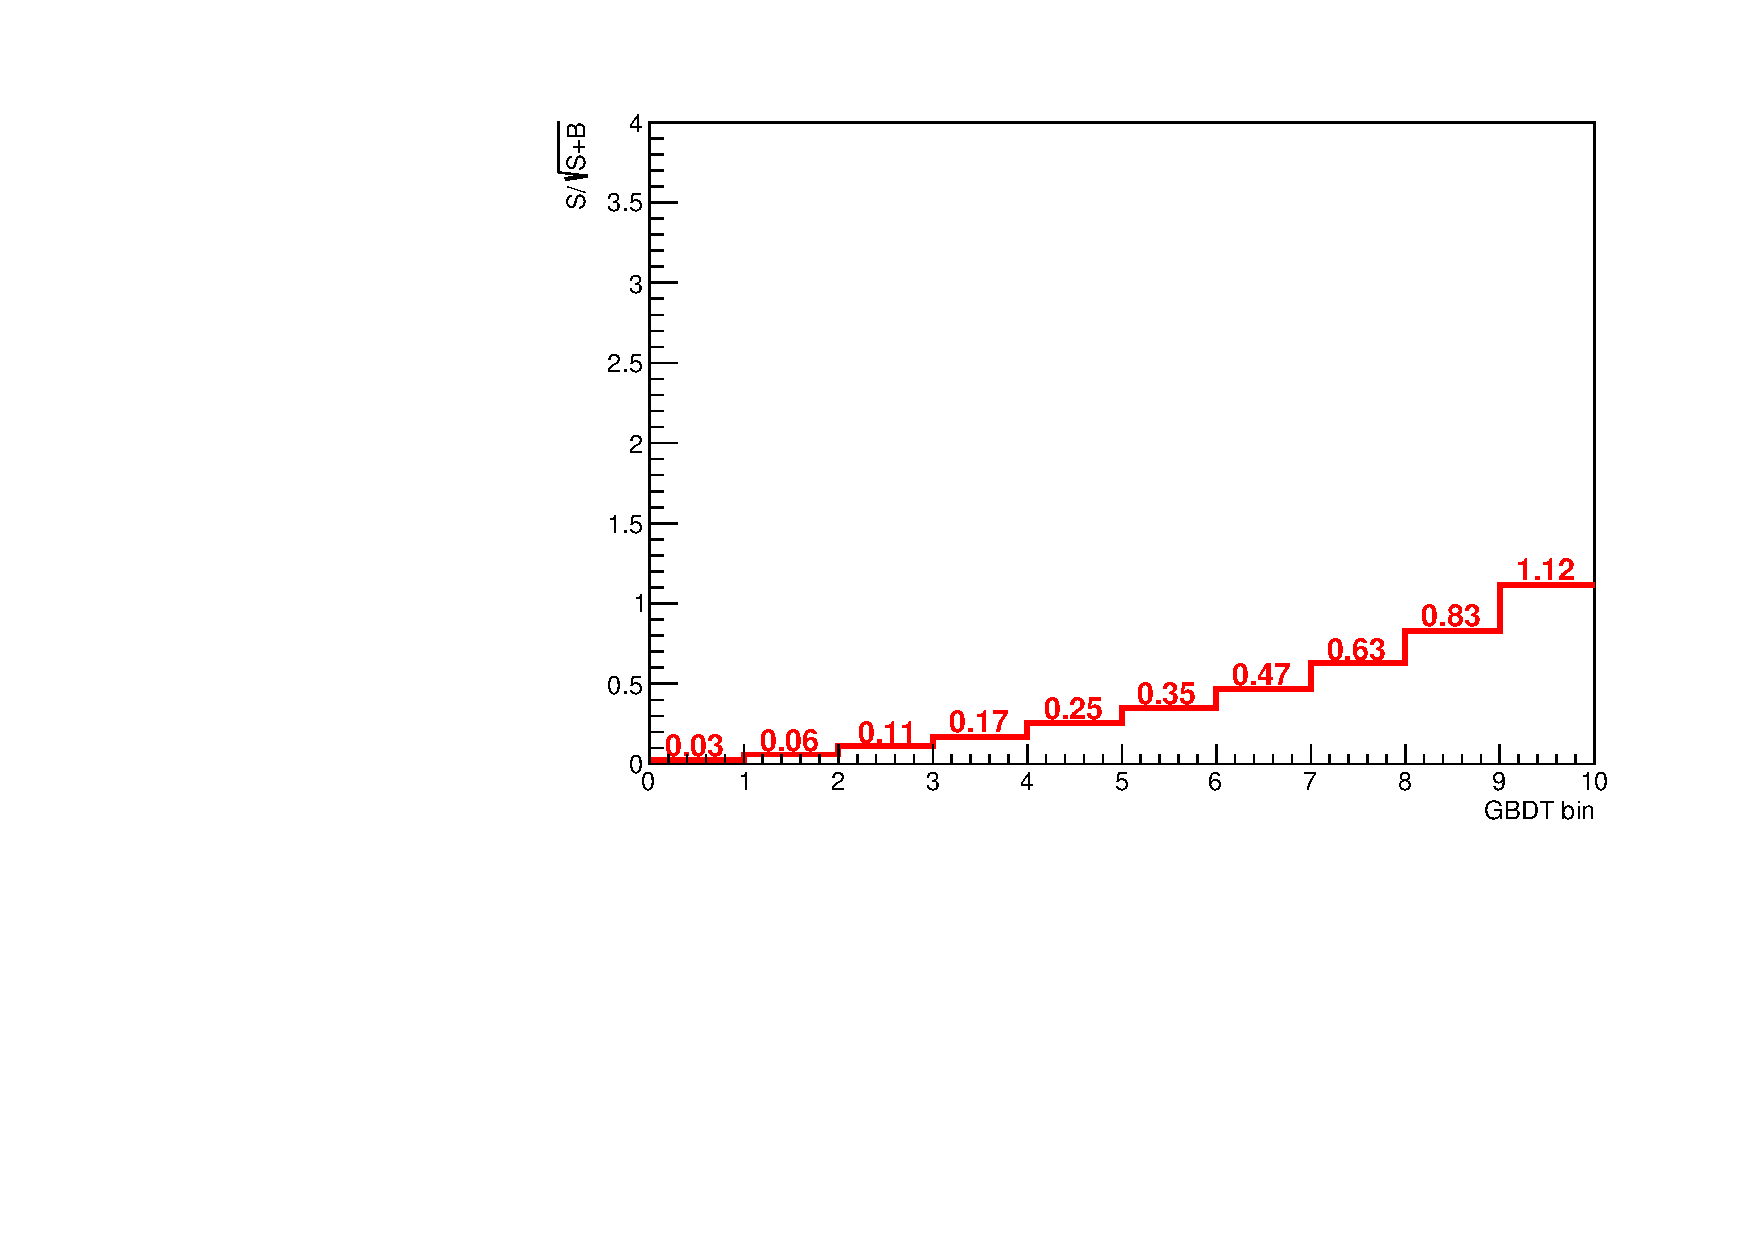
\includegraphics[width=.9\textwidth]{Chapters/CH6/figures/GBDT_smt}
		\label{fig:yields:sr3_smt_bdt}} \qquad
	\subfigure[\DLrc selection]{
		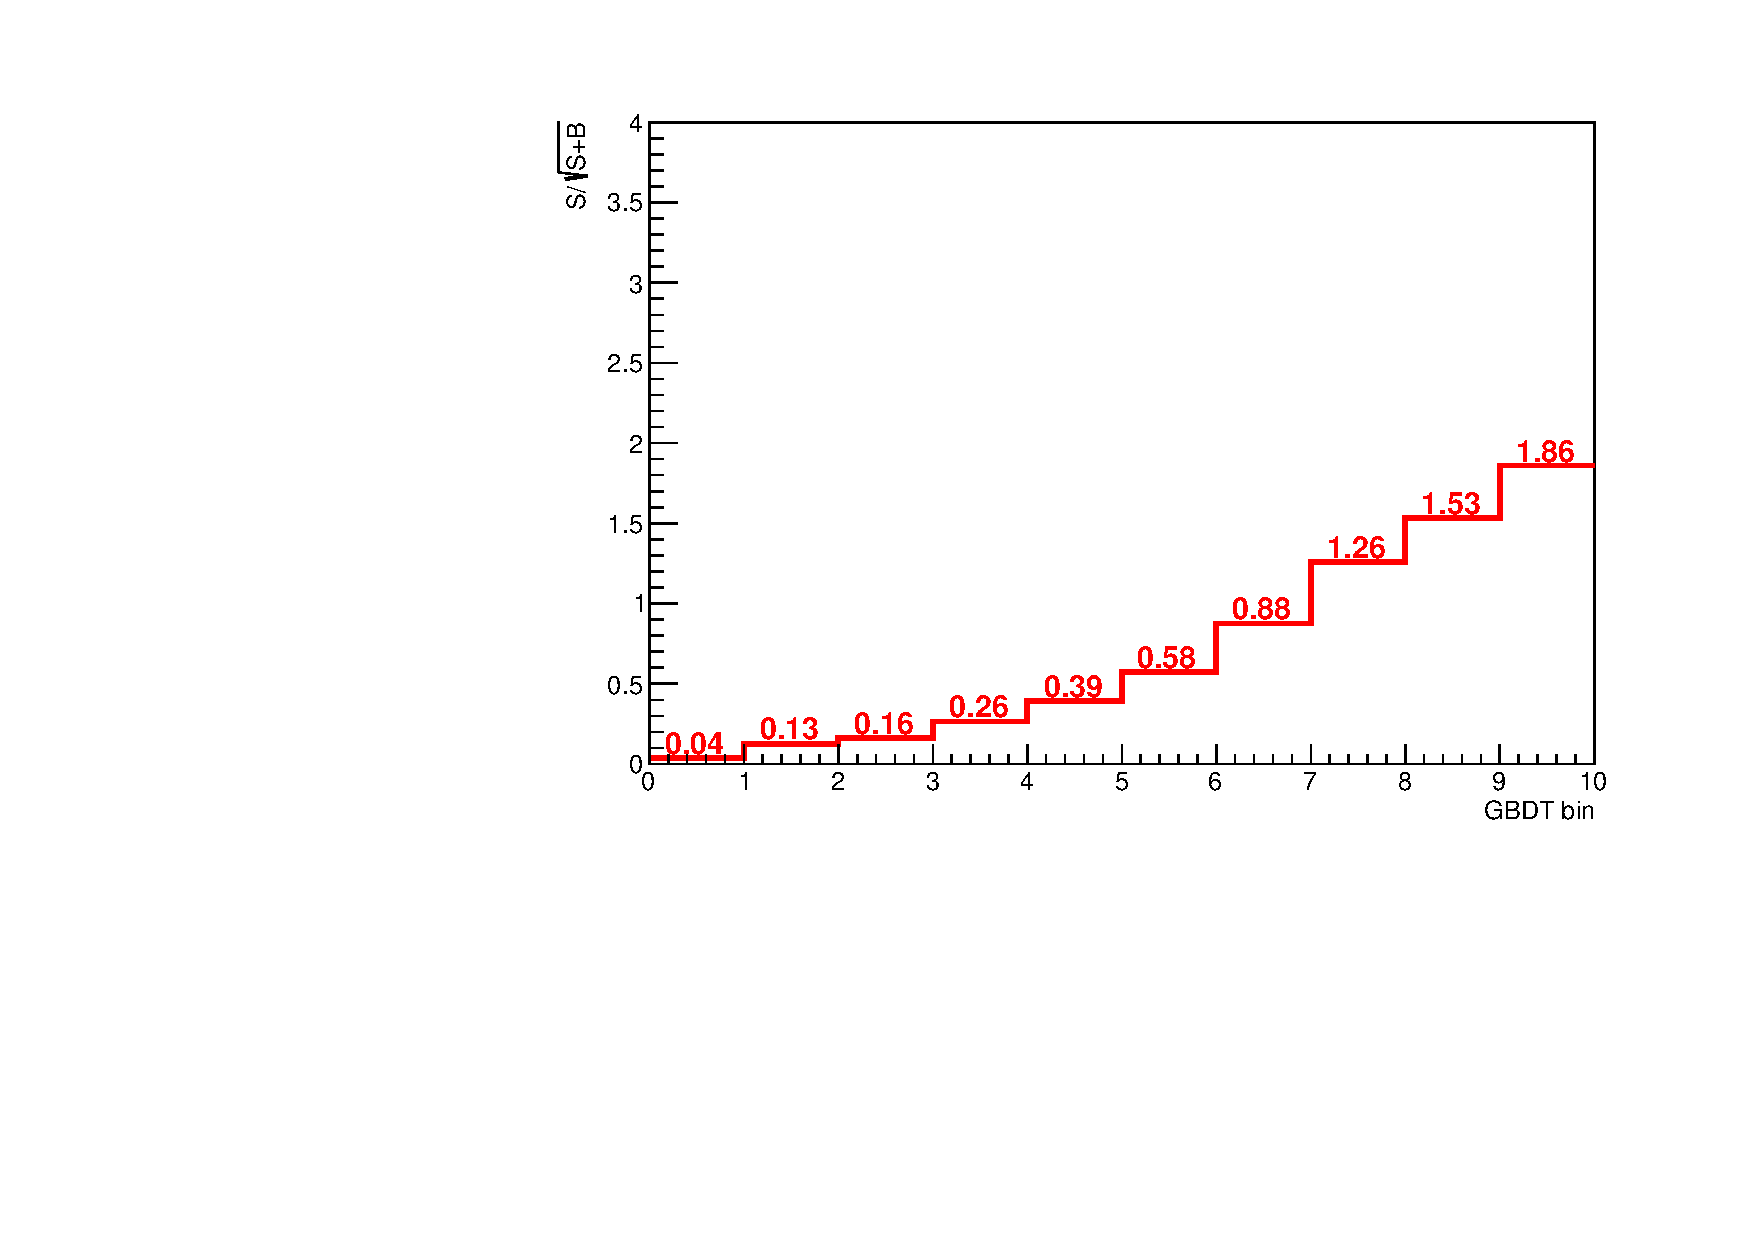
\includegraphics[width=.9\textwidth]{Chapters/CH6/figures/GBDT_dl1rc}
		\label{fig:yields:sr3_dl1rc_bdt}} \\
	\caption{Values of \ssplusb for each bin of the GBDT discriminant for ~\subref{fig:yields:sr3_smt_bdt} SMT selection and ~\subref{fig:yields:sr3_dl1rc_bdt} for \DLrc selection. 	}%
	\label{fig:yields:sr3_bdt}
\end{figure}

\begin{table}[!h]
	\centering
	\small
\begin{tabular}{|l|c|c|c|c|c|} 
	\hline 
	Sample 			       & Bin 6            & Bin 7            & Bin 8             & Bin 9           & Bin 10          \\ 
	\hline                 
	Others & 0.46 $\pm$ 0.42 & 0.91 $\pm$ 0.63 & 0.04 $\pm$ 0.05 & 0.02 $\pm$ 0.05 & 0.00 $\pm$ 0.05 \\ 
	$Z$ + jets & 0.18 $\pm$ 0.17 & 0.00 $\pm$ 0.17 & 0.26 $\pm$ 0.23 & 0.40 $\pm$ 0.28 & 0.21 $\pm$ 0.36 \\ 
	$t\bar{t}+tW$ & 1.07 $\pm$ 0.28 & 0.61 $\pm$ 0.24 & 0.43 $\pm$ 0.23 & 0.59 $\pm$ 0.22 & 0.16 $\pm$ 0.21 \\ 
	$tZq$ & 2.80 $\pm$ 0.13 & 2.08 $\pm$ 0.12 & 2.10 $\pm$ 0.11 & 1.48 $\pm$ 0.10 & 1.03 $\pm$ 0.08 \\ 
	$VV$ + HF & 6.11 $\pm$ 0.19 & 4.65 $\pm$ 0.20 & 2.85 $\pm$ 0.14 & 1.70 $\pm$ 0.11 & 0.82 $\pm$ 0.09 \\ 
	$VV$ + LF & 2.67 $\pm$ 0.13 & 1.56 $\pm$ 0.10 & 0.62 $\pm$ 0.07 & 0.15 $\pm$ 0.04 & 0.06 $\pm$ 0.01 \\ 
	$t\bar{t}H+t\bar{t}W$ & 0.55 $\pm$ 0.05 & 0.40 $\pm$ 0.04 & 0.25 $\pm$ 0.04 & 0.15 $\pm$ 0.03 & 0.06 $\pm$ 0.02 \\ 
	$t\bar{t}Z+tWZ$ & 7.83 $\pm$ 0.23 & 6.43 $\pm$ 0.21 & 4.65 $\pm$ 0.18 & 3.12 $\pm$ 0.15 & 1.62 $\pm$ 0.12 \\ 
	\hline 
	Total bkg & 21.67 $\pm$ 0.63 & 16.65 $\pm$ 0.77 & 11.21 $\pm$ 0.43 & 7.60 $\pm$ 0.42 & 3.97 $\pm$ 0.45 \\ 
	\hline 
	Signal & 1.69 $\pm$ 0.03 & 2.02 $\pm$ 0.03 & 2.31 $\pm$ 0.03 & 2.66 $\pm$ 0.03 & 2.93 $\pm$ 0.03 \\ 
	\hline 
	$S/B$ & 0.08 & 0.12 & 0.21 & 0.35 & 0.74 \\ 
	$S/\sqrt{S+B}$ & 0.35 & 0.47 & 0.63 & 0.83 & 1.12 \\ 
	\hline 
\end{tabular} 
	\caption{Values of \ssplusb for each bin of the GBDT discriminant for the SMT selection.}%
\label{tab:yields:sr3_smt_bdt}
\end{table}

\begin{table}[!h]
	\centering
	\small
	\begin{tabular}{|l|c|c|c|c|c|} 
		\hline 
		Sample 			       & Bin 6            & Bin 7           & Bin 8           & Bin 9           & Bin 10          \\ 
		\hline                 
		Others 			       & 0.03  $\pm$ 0.03 & 0.01 $\pm$ 0.03 & 0.02 $\pm$ 0.03 & 0.00 $\pm$ 0.03 & 0.00 $\pm$ 0.03 \\
		$Z$ + jets             & 0.36  $\pm$ 0.29 & 0.06 $\pm$ 0.07 & 0.00 $\pm$ 0.07 & 0.21 $\pm$ 0.24 & 0.00 $\pm$ 0.07 \\
		$t\bar{t}+tW$          & 0.64  $\pm$ 0.15 & 0.17 $\pm$ 0.08 & 0.16 $\pm$ 0.08 & 0.14 $\pm$ 0.07 & 0.17 $\pm$ 0.09 \\
		$tZq$ 			       & 1.80  $\pm$ 0.10 & 1.37 $\pm$ 0.08 & 0.76 $\pm$ 0.06 & 0.46 $\pm$ 0.04 & 0.27 $\pm$ 0.03 \\
		$VV$ + HF              & 2.51  $\pm$ 0.13 & 1.86 $\pm$ 0.12 & 0.97 $\pm$ 0.07 & 0.53 $\pm$ 0.06 & 0.19 $\pm$ 0.03 \\
		$VV$ + LF              & 0.25  $\pm$ 0.04 & 0.24 $\pm$ 0.05 & 0.08 $\pm$ 0.02 & 0.06 $\pm$ 0.03 & 0.00 $\pm$ 0.00 \\
		$t\bar{t}H+t\bar{t}W$  & 0.36  $\pm$ 0.04 & 0.37 $\pm$ 0.04 & 0.30 $\pm$ 0.03 & 0.17 $\pm$ 0.03 & 0.10 $\pm$ 0.02 \\
		$t\bar{t}Z+tWZ$        & 6.77  $\pm$ 0.22 & 4.53 $\pm$ 0.18 & 2.60 $\pm$ 0.14 & 1.38 $\pm$ 0.09 & 0.66 $\pm$ 0.07 \\
		\hline                                                                                                           
		Total bkg              & 12.74 $\pm$ 0.43 & 8.60 $\pm$ 0.26 & 4.88 $\pm$ 0.20 & 2.97 $\pm$ 0.28 & 1.40 $\pm$ 0.14 \\
		\hline                                                                                                           
		Signal                 & 2.23  $\pm$ 0.12 & 2.98 $\pm$ 0.14 & 3.69 $\pm$ 0.16 & 4.07 $\pm$ 0.16 & 4.54 $\pm$ 0.17 \\
		\hline                 
		$S/B$                  & 0.17             & 0.35            & 0.76            & 1.37            & 3.24            \\
		$S/\sqrt{S+B}$         & 0.58             & 0.88            & 1.26            & 1.53            & 1.86       \\
		\hline
	\end{tabular} 
	\caption{Values of \ssplusb for each bin of the GBDT discriminant for the \DLrc selection.}%
	\label{tab:yields:sr3_dl1rc_bdt}
\end{table}



